\documentclass[output=paper]{langscibook}
\ChapterDOI{10.5281/zenodo.15148182}
\author{Xuan Guan\orcid{}\affiliation{University of Oregon}}
\title{Uvularization in Queyu phonology}
\abstract{This chapter examines uvularization in Queyu, a Qiangic language within the Ti\-beto-Burman language family. Queyu contains a series of uvularized vowels characterized by the constriction of the styloglossus and other muscles which draw the tongue dorsum towards the uvula (\citealt{EvansEtAl2016}: 1). Uvularity in Queyu can spread leftwards across morpheme boundaries and can trigger a uvular allophone of a preceding velar consonant. In addition to describing relevant phonological phenomena associated with uvularized vowels, this chapter provides an overview of current literature on uvularization and other similar vowel qualities in closely-related languages, and discusses possible origins of this unique phenomenon. As different labels are used for similar vowel qualities in the literature, this chapter draws attention to the need for detailed acoustic studies and terminological systemization.
\keywords{Qiangic, uvularization, Queyu}}
\IfFileExists{../localcommands.tex}{
  \addbibresource{../localbibliography.bib}
  \usepackage{tabularx, multicol, multirow, longtable}
\usepackage{url}
\urlstyle{same}

\usepackage{orcidlink}
\definecolor{orcidlogocol}{cmyk}{0,0,0,1}
\RenewDocumentCommand{\LinkToORCIDinAffiliations}{ +m }
  {%
    \orcidlink{#1}\,%
  }
\SetupAffiliations{orcid placement=before}

\usepackage{siunitx}
\sisetup{detect-weight=true, detect-family=true, group-digits=none}

\usepackage{mathtools}
\usepackage{langsci-optional}
\usepackage{langsci-lgr}
\usepackage{langsci-gb4e}

\usepackage{stmaryrd}
\usepackage[capitalize]{cleveref}
\babelfont[macedonian]{rm}[Language=Macedonian,ItalicFont=LibertinusSerif-Italic.otf]{LibertinusSerif-Regular.otf}
\usepackage{eqparbox}
\usepackage[autostyle]{csquotes}
\usepackage[linguistics]{forest}

\usetikzlibrary{positioning, matrix}
\usepackage[glosses,inline]{leipzig}
\PassOptionsToPackage{xindy,toc,nopostdot}{glossaries}
\usepackage{glossary-inline}
\setglossarystyle{inline}
\makeglossaries

\usepackage{phonrule}
\usepackage{threeparttable}


\usepackage{textcomp,gensymb}


\usepackage[preservefont]{tipauni}

\usepackage[normalem]{ulem}

\usepackage{enumitem} %so lists aren't ugly
	
\usepackage{threeparttable}	%allows tables with tablenotes. note marks: †‡
	\makeatletter 
	\g@addto@macro\TPT@defaults{\footnotesize} 
	\makeatother

\usepackage{colortbl}
	\definecolor{Pink}{rgb}{0.96, 0.76, 0.76} 
	\definecolor{PaleBlue}{rgb}{0.67, 0.9, 0.93}
	\definecolor{carolinablue}{rgb}{0.6, 0.73, 0.89}
	\definecolor{goldenyellow}{rgb}{1.0, 0.87, 0.0}
	\definecolor{Orange}{rgb}{1.0, 0.66, 0.07}
	\definecolor{puce}{rgb}{0.8, 0.53, 0.6}
	\definecolor{turquoisegreen}{rgb}{0.63, 0.84, 0.71}


% add all extra packages you need to load to this file
\usepackage{langsci-textipa}
\usepackage{vowel}
\usepackage{textgreek}

% \usepackage{langsci-branding}
% \usepackage{subcaption}
\usepackage{subfigure}

\usepackage{tabto}


\usetikzlibrary{tikzmark}
\usepackage{pgfplots}


\newfontfamily\tibetan{NotoSerifTibetan-Regular.ttf}
\usepackage{langsci-branding}
\usepackage{hyphenat}

\usepackage{accents}

  \renewcommand{\lsChapterFooterSize}{\footnotesize}

\makeatletter
\let\thetitle\@title
\let\theauthor\@author
\makeatother

\newcommand{\togglepaper}[1][0]{
   \bibliography{../localbibliography}
   \papernote{\scriptsize\normalfont
     \theauthor.
     \titleTemp.
     To appear in:
     Natalia Kuznetsova, Cormac Anderson \& Shelece Easterday (ed.).
     Rarities in phonetics and phonology.tex.
     Berlin: Language Science Press. [preliminary page numbering]
   }
   \pagenumbering{roman}
   \setcounter{chapter}{#1}
   \addtocounter{chapter}{-1}
}

\newbool{bookcompile}
\booltrue{bookcompile}
\newcommand{\bookorchapter}[2]{\ifbool{bookcompile}{#1}{#2}}

\newcommand{\textarab}[1]{\RL{\arabicfont #1}}

\newcommand\mb[1]{\eqparbox[t]{examples}{#1}\hspace{1em}}
\newcommand\mbi[1]{\mb{#1}}
\newcommand{\twe}[3]{\mbi{#1}\eqparbox[t]{orths}{\emph{#2}}\hspace{1em}`#3'\hspace{1em}} % three-way example
\providecommand\glottocode[1]{[\href{https://glottolog.org/resource/languoid/id/#1}{#1}]}
\newcommand{\phonreal}[1]{\ensuremath{\llbracket}#1\ensuremath{\rrbracket}}

\DeclareRobustCommand\dash{\unskip\nobreak\thinspace\textendash\allowbreak\thinspace\ignorespaces}

\forestset{minus/.style={edge label={node[midway, left] {\ensuremath{-}\hspace*{2mm}}}},
plus/.style={edge label={node[midway, right] {\hspace*{2mm}\ensuremath{+}}}}}
\providecommand\ipa[1]{#1}


\newcommand{\tone}[1]{\textsuperscript{#1}}

\newcommand{\orthog}[1]{\textit{#1}}
\newcommand{\gloss}[1]{`#1'}

\newcommand{\glottolog}[1]{\texttt{\href{https://glottolog.org/resource/languoid/id/#1}{#1}}}

\newcolumntype{O}{>{\itshape }l<{}}
\newcolumntype{G}{>{`}l<{'}}

\newcounter{tabsubcounter}
\newcommand{\tablecounter}{\setcounter{tabsubcounter}{0}}
\newcommand{\TC}{\stepcounter{tabsubcounter}\alph{tabsubcounter}.}

\usetikzlibrary{chains,positioning,calc,decorations.markings}
\tikzset{
	seg/.style={text height=0.6em, text depth=0.3em},
	moraic-structure/.style={xscale=0.6,yscale=1.1, text height=0.65em,text depth=0.25em},
 }

%05_Culhane_Edwards
%%%%%%%%%%%%%%%%%%%%%%%%%%%%%%%%
%%	Symbols and Characters  	%%
%%%%%%%%%%%%%%%%%%%%%%%%%%%%%%%% αβσµ

\newcommand{\tl}{\char`~}						%middle tilde ~
\renewcommand{\Q}{\textquotesingle}		%straight apostrophe444
\newcommand{\ra}{→} 								%right arrow ->
\newcommand{\0}{∅} 									%zero symbol
\newcommand{\gap}{\textunderscore} 	%underscore
%\renewcommand{\j}{ʤ}								%dezh digraph
\newcommand{\syll}{σ}								%lowercase sigma medial form
\newcommand{\wrd}{ω}								%lowercase omega
\newcommand{\ft}{φ}									%lowercase phi
\newcommand{\gw}{gʷ}								%g with superscript w
\newcommand{\B}{β}									%voiced bilabial fricative
\newcommand{\hp}{\hphantom}					%space equal to width of argument
\newcommand{\it}{\textit}	%italics

%%%%%%%%%%%%%%%%%%%%%%%%%%%%%%%%
%%	Font Styles & Formatting	%%
%%%%%%%%%%%%%%%%%%%%%%%%%%%%%%%%

\definecolor{DarkBlue}{RGB}{0,0,130}										%dark blue colour
% \newcommand{\ve}[1]{\textcolor{DarkBlue}{\textit{#1}}}	%vernacular text
\newcommand{\ve}[1]{{\textit{#1}}}	%vernacular text
\definecolor{DarkRed}{RGB}{150,0,0}											%dark red colour
% \newcommand{\tbr}[1]{\textcolor{DarkRed}{\textbf{#1}}}	%Bold red text
\newcommand{\tbr}[1]{{\textbf{#1}}}	%Bold red text
%\renewcommand{\it}{\textit}																%italics
\newcommand{\tsc}{\textsc}															%small caps
\newcommand{\sub}{\textsubscript}												%subscript
\newcommand{\su}{\textsuperscript}											%superscript

%%%%%%%%%%%%%%%%%%%%%%%%%%%%%%%%%%%%%%%%%%%%%%%%%%%%
%% Tables %% Tables %% Tables %% Tables %% Tables %%
%%%%%%%%%%%%%%%%%%%%%%%%%%%%%%%%%%%%%%%%%%%%%%%%%%%%

% \newcommand{\mc}{\multicolumn}									%multicolumn
% \newcommand{\st}[1]{\setlength{\tabcolsep}{#1}}	%reduce column width in tables
%
%%%%%%%%%%%%%%%%%%%%%%%%%%%%%%%%
%%    Cross   References      %%
%%%%%%%%%%%%%%%%%%%%%%%%%%%%%%%%

% \def\Plus{\texttt{+}}
% \def\Minus{\texttt{-}}
% \newcommand{\GS}{ʔ}
% \def\SH{ʃ}
% \newcommand{\TSH}{ʧ}
% \def\ZH{ʒ}
% \def\DZH{ʤ}
% \def\:{ː}
% \def\UP{\textsuperscript}
% \def\rs{ʂ}
% \newcommand{\rn}{ɳ}
% \def\rt{ʈ}
% \def\tllr{ɺ}
% \newcommand{\Bb}{β}
% \def\Eps{ɛ}
% \def\Oo{ɔ}
% \def\Gm{ɣ}
% \def\NG{ŋ}
% \def\barU{ʉ}
\newcommand{\CM}{\ding{51}}
\newcommand{\XM}{\ding{53}}
% \newcommand{\tap}{ɾ}
% \def\darkL{ɫ}
% \def\schwa{ə}
%
% \def\BUL{\textbullet}


%%%%%%%%%%%%%%
%					%
%	Secondaries		%
%					%
%%%%%%%%%%%%%%
%	Post
\newcommand{\Post}[2]{#1\textsuperscript{#2}}
%	Pre
\newcommand{\Pre} [2] {\textsuperscript{#1}#2}
%	Undertilde
\newcommand{\utilde}[1]{\ensuremath{\smash{\underset{\mathclap{\sim}}{\text{#1}}}}}
%	Devoiced
% \newcommand{\VCLS}[1]{\textsubring{#1}}
%%%%%%%%%%%
%				%
%	Definitions		%
%	Markup		%
%				%
%%%%%%%%%%%
% \def\->{$\rightarrow$}
% \def\__{\underline{\hspace{1em}}}
\def\NoPoss{\cellcolor{gray!30}}

\newcommand{\VOICELESS}{\textsc{voiceless}}
\newcommand{\VOICED}{\textsc{voiced}}
\newcommand{\tablenote}[2][1]{\parbox{#1\textwidth}{\footnotesize\raggedright #2}}

\newcommand{\appref}[1]{Appendix~\ref{#1}}
\renewcommand{\sectref}[1]{Section~\ref{#1}}


\newcommand{\dobuibox}[5]{#1\\[-1.1em]
\hspace*{-.8cm}
 \begin{tabularx}{.9\textwidth}{@{}lQQ@{}}
       &  {oral} &  {nasal} \\
       \midrule
     {controlled} &\parbox[t]{4cm}{\raggedright  #2} & \parbox[t]{4cm}{\raggedright #3} \\
     \tablevspace
     {ballistic} &\parbox[t]{4cm}{\raggedright  #4} & \parbox[t]{4cm}{\raggedright  #5} \\
 \end{tabularx}
}

\newfontfamily\VdottildeFont{LibertinusVdottilde.otf}

\newcommand{\Vdottilde}{{\VdottildeFont V̰̣}}

% \renewcommand{\keywords}[1]{\textbf{#1}}
 
  %% hyphenation points for line breaks
%% Normally, automatic hyphenation in LaTeX is very good
%% If a word is mis-hyphenated, add it to this file
%%
%% add information to TeX file before \begin{document} with:
%% %% hyphenation points for line breaks
%% Normally, automatic hyphenation in LaTeX is very good
%% If a word is mis-hyphenated, add it to this file
%%
%% add information to TeX file before \begin{document} with:
%% %% hyphenation points for line breaks
%% Normally, automatic hyphenation in LaTeX is very good
%% If a word is mis-hyphenated, add it to this file
%%
%% add information to TeX file before \begin{document} with:
%% \include{localhyphenation}
\hyphenation{
    af-fri-cates
    al-ve-o-pal-a-tal
    Ama-nu-ban
    Ara-wak-an
    Árna-son
    Ber-ber
    can-di-dates
    Cam-er-oon
    Chi-nan-tec
    Chir-ko-va
    Crai-o-ve-a-nu
    di-chot-o-my
    Ec-ua-do-rian
    Ec-ua-dor
    elec-tro-glot-to-gra-phy
    Faro-ese
    Ike-ma
    Kuznet-sova
    Mes-kwa-ki
    Mio-ma-fo
    mono-mor-aic
    Ne-ca-xa
    Oto-man-gue-an
    par-a-digm
    post-as-pi-rat-ed
    post-as-pi-ra-tion
    pre-as-pi-rat-ed
    pre-as-pi-ra-tion
    pros-o-dic
    pros-o-dies
    re-con-struc-table
    Sheh-ret
    Svan-tes-son
    Ta-ras-can
    Tórs-havn
    Ural-ic
    epen-the-sis
    Anin-dil-yak-wa
    Mi-nyag
    Na-ka-ma
}

\hyphenation{
    af-fri-cates
    al-ve-o-pal-a-tal
    Ama-nu-ban
    Ara-wak-an
    Árna-son
    Ber-ber
    can-di-dates
    Cam-er-oon
    Chi-nan-tec
    Chir-ko-va
    Crai-o-ve-a-nu
    di-chot-o-my
    Ec-ua-do-rian
    Ec-ua-dor
    elec-tro-glot-to-gra-phy
    Faro-ese
    Ike-ma
    Kuznet-sova
    Mes-kwa-ki
    Mio-ma-fo
    mono-mor-aic
    Ne-ca-xa
    Oto-man-gue-an
    par-a-digm
    post-as-pi-rat-ed
    post-as-pi-ra-tion
    pre-as-pi-rat-ed
    pre-as-pi-ra-tion
    pros-o-dic
    pros-o-dies
    re-con-struc-table
    Sheh-ret
    Svan-tes-son
    Ta-ras-can
    Tórs-havn
    Ural-ic
    epen-the-sis
    Anin-dil-yak-wa
    Mi-nyag
    Na-ka-ma
}

\hyphenation{
    af-fri-cates
    al-ve-o-pal-a-tal
    Ama-nu-ban
    Ara-wak-an
    Árna-son
    Ber-ber
    can-di-dates
    Cam-er-oon
    Chi-nan-tec
    Chir-ko-va
    Crai-o-ve-a-nu
    di-chot-o-my
    Ec-ua-do-rian
    Ec-ua-dor
    elec-tro-glot-to-gra-phy
    Faro-ese
    Ike-ma
    Kuznet-sova
    Mes-kwa-ki
    Mio-ma-fo
    mono-mor-aic
    Ne-ca-xa
    Oto-man-gue-an
    par-a-digm
    post-as-pi-rat-ed
    post-as-pi-ra-tion
    pre-as-pi-rat-ed
    pre-as-pi-ra-tion
    pros-o-dic
    pros-o-dies
    re-con-struc-table
    Sheh-ret
    Svan-tes-son
    Ta-ras-can
    Tórs-havn
    Ural-ic
    epen-the-sis
    Anin-dil-yak-wa
    Mi-nyag
    Na-ka-ma
}
 
  \togglepaper[11]%%chapternumber
}{}

\begin{document}
\maketitle

\section{Introduction}\label{sec:guan:1}

This chapter examines the phonological characteristics of Queyu (Qiangic < Ti\-beto-Burman (TB), ISO 639: qvy) in the context of nearby languages. The Queyu language contains an unusual combination of elaborate onset clusters and highly reduced codas. While uvular consonants and uvularized vowels are typologically rare among languages of the world, they are common in the region where Queyu is spoken. Uvular consonants and uvularized vowels are related to each other in Queyu. Uvular consonants only occur before uvularized vowels, suggesting that uvular and velar consonants are allophones. This chapter argues that in Queyu, the appearance of uvular consonants is triggered by uvularized vowels. Vowel qualities similar to what is described here as uvularized are mentioned in descriptions and analyses of related neighboring languages, where they are variously termed as pharyngealization, velarization,\footnote{This is not to be confused with the “highly velarized allophone of /u/” mentioned in \textcitetv{chapters/10_HugteEtAl}, which is associated with fricative vowels, another rare phenomenon that is also present in Qiangic languages.} tenseness, and rhotacization (\citealt{Gong2020}: 193, \citealt{Chirkova2024}: 734). The similarities among these vowel qualities have been noted by several authors (\citealt{Evans2006a}: 94, \citealt{Evans2006b}: 737, \citealt{Suzuki2011}: 492, \citealt{Suzuki2013}: 30, \citealt{Gong2020}: 194). In this work, I withhold judgement about whether these various vowel qualities represent differing descriptions of a common set of acoustic features which have yet to be systematically defined, or are indeed truly distinct. These studies show that the marked vowels in question differ from plain vowels in different ways across the languages they are identified in. While some marked vowels have lower F2, others may have higher F1 and/or F3, yet all marked vowels can be implicated in similar phonological processes, like vowel harmony (\citealt{LinEtAl2012}, \citealt{EvansEtAl2016}, \citealt{Way2018}, \citealt{ChiuSun2020}). In addition to describing rare phonological phenomena in Queyu and the spreading of this unusual vowel quality within a word as areal features, this chapter looks at Queyu phonology from both comparative and typological perspectives, and examines the possible origins of uvularized vowels.

\sectref{sec:guan:2} briefly introduces Queyu and its current available literature, then provides a description of relevant phonological phenomena. \sectref{sec:guan:3} presents a typological overview of uvularized vowels and related phonological processes within the Qiangic branch and discusses the possible origins of uvularization. \sectref{sec:guan:4} concludes the chapter.

\section{Introduction to Queyu and Queyu phonology}\label{sec:guan:2}
\subsection{The Queyu language and Qiangic branch}\label{sec:guan:2.1}

Queyu is a Tibeto-Burman (TB) language spoken in Ganzi Tibetan Autonomous Prefecture, Sichuan Province, China. Though the language’s 6,000{--}7,000 speakers are ethnic Tibetans (\citealt{Lu1985}: 67, \citealt{Wang1991}: 46), Queyu belongs to the Qiangic branch rather than Tibetic. The subgrouping of Queyu and its related languages is still under debate. For example, \citet[4]{Sun2016} puts thirteen languages under the Qiangic branch, while \citet{JacquesMichaud2011} propose a Na-Qiangic sub-branch containing 25 languages. In Sun's (\citeyear{Sun2016}) classification, Queyu, Muya (Minyag, Munya), Pumi (Prinmi), Tangut (Xixia), Qiang (Rma), and Zhaba (nDra\-pa) belong to the Central sub-branch, while Shixing (Shuhi), Namuyi, Ersu and Gui\-qiong belong to a Southern sub-branch, and Rgyalrong, Ergong (Stau, Daofu, Horpa), and Lavrung (Khroskyabs) belong to a Northern sub-branch.\footnote{Alternative names and spellings of a language that are used in various literature are given in parentheses.} Though there is controversy regarding the Qiangic grouping \citep{Chirkova2012}, morphological evidence supports Sun’s proposed Northern sub-branch as a group. This group is often referred to as Rgyalrongic in the literature (\citealt{Sun2000a,Sun2000b}).

Language data from Qiang, Tangut, Khroskyabs, Rgyalrong, and Tibetan will be presented in the discussion on the origins of uvularization given in \sectref{sec:guan:3.5}. In TB literature, it is a common practice to use the place name (such as village/town/county name) where a specific language/variety is spoken in labeling different languages or varieties within a language (e.g. Puxi Stau, Xiaoyili Khroskyabs, Mawo Qiang). This chapter follows this convention when citing data from other sources.

  The literature reports that Queyu speakers mainly reside in the counties of Xinlong, Litang, and Yajiang (\citealt{Lu1985}: 67, \citealt[46]{Wang1991}, \citealt[159]{Sun2001}, \citealt[77]{Nishida2008}). My primary interest in this study is the Queyu variety spoken in Yajiang County, Pubarong Town. This variety is hence referred to as “Pubarong Queyu”.  

Compared to other languages in the proposed Qiangic group, Queyu has received relatively little attention and is one of the least studied languages in the area. To date, there are only two published grammar sketches on Queyu varieties: \citet{Lu1985} introduces basic information on the Queyu variety spoken in Yajiang County, Tuanjie Town (now renamed Gala Town), and \citet{Wang1991} describes the Queyu variety in Xinlong County, Youlaxi Town. Partial descriptions of other Queyu varieties are also available. \citet{Nishida2008} discusses the phonology of the Queyu spoken in Litang County, Rongba Town. \citet{Zheng2023} is a more detailed description and analysis of the Rongba Queyu phonology. \citet{NaganoPrins2013} provide a wordlist with 407 words from Yajiang County, Gala Town. Recently a moribund variety of Queyu was identified near Yajiang County in Lhagang, Kangding County (\citealt{SuzukiWangmo2016}, \citealt{SuzukiWangmo2018}, \citealt{SuzukiWangmo2019}).

The description and analysis of Pubarong Queyu presented in this chapter is based on data collected through fieldwork undertaken from 2018--2021. I worked mainly with Pubarong Queyu speakers from the village of Suoyi. The villages of Pubarong are divided into \textit{lə̀ndʒə́} and \textit{vɘ̀ndʒə́} based on their locations in relation to the Yalong River, with the \textit{lə̀ndʒə́} villages upstream and the \textit{vɘ̀ndʒə́} villages downstream. Suoyi belongs to the downstream \textit{vɘ̀ndʒə́} group. The location of Suoyi Village is labeled with a star in the map below. Other Pubarong Queyu speaking villages are labeled by a pin.

 
\begin{figure}
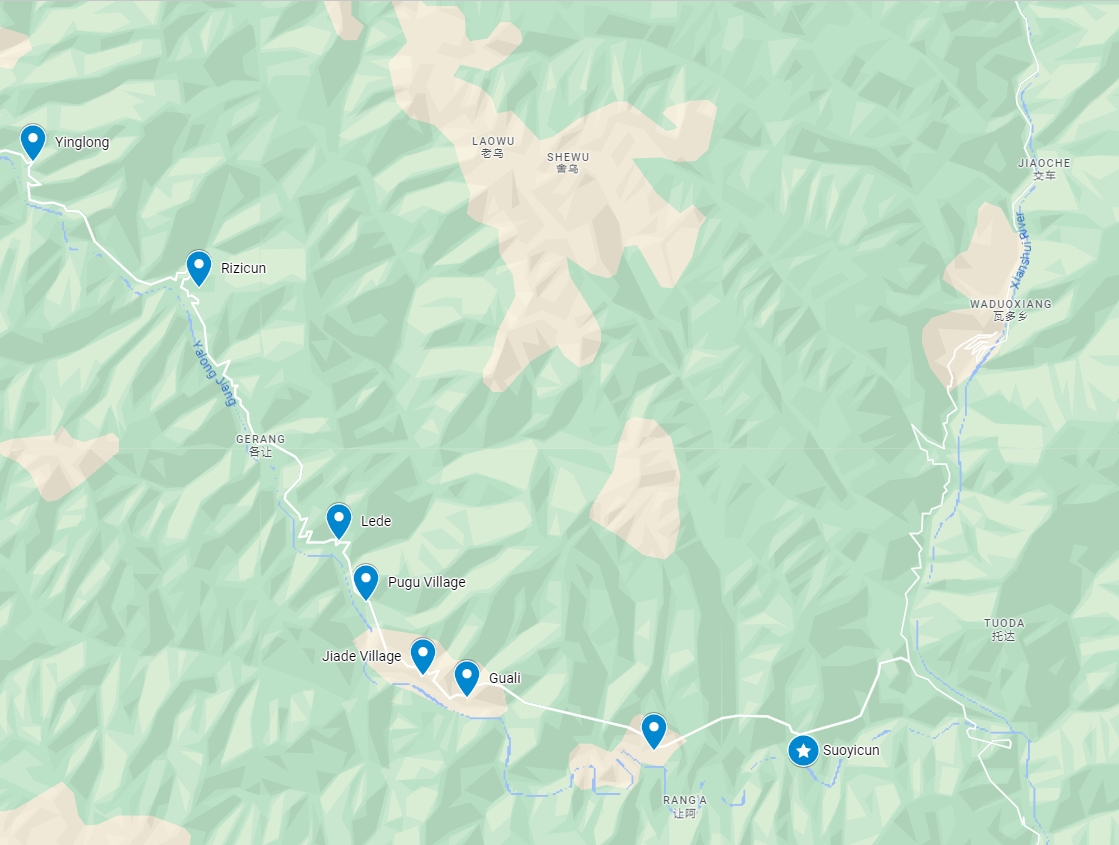
\includegraphics[width=\textwidth]{figures/Guan-img001.png}
\caption{The location of Suoyi Village in relation to other Pubarong Queyu speaking villages along the Yalong River} 
\label{fig:guan:1}
\end{figure}

\subsection{Phonological sketch of Queyu}\label{sec:guan:2.2}

\subsubsection{Phoneme inventory}\label{sec:guan:2.2.1}


There has not been much work on Queyu varieties from a phonological perspective. The current study is the first description of Pubarong Queyu variety. There are forty-three consonants in Pubarong Queyu, which are given in \tabref{tab:guan:1}.

\begin{sidewaystable}
\caption{Consonant inventory of Pubarong Queyu}
\label{tab:guan:1}
\begin{tabularx}{\textwidth}{Xlllllll@{}ll}
\lsptoprule
{} &   & {Bilabial} & {Labio-dental} & {Alveolar} & {Retroflex} & {Palatal} & {Velar}\\
\midrule
{{Plosive}} & {voiceless aspirated} & {pʰ} &   & {tʰ} &   &   & {kʰ [kʰ, qʰ]} &  \\
& {voiceless unaspirated} & {p [p, ɸ]} &   & {t} &   &   & {k [k, q]} &  \\
& {Voiced} & {b [b, β]} &   & {d} &   &   & {ɡ [ɡ, ɢ]} &  \\
{{Affricate}} & {voiceless aspirated} &   &   & {tsʰ} & {ʈʂʰ}  & {tʃʰ} &   &  \\
& {voiceless unaspirated} &   &   & {ts} & {ʈʂ} & {tʃ} &   &  \\
& {Voiced} &   &   & {dz} & {ɖʐ} & {dʒ} &   &  \\
{{Fricative}} & {voiceless unaspirated} &  &   & {s} & {ʂ} & {ʃ} & {x [x, χ, h]} & &\\
& {voiceless aspirated} &   &   & {sʰ} & {ʂʰ} & {ʃʰ} & {xʰ~} &  \\
& {Voiced} &  & {v} & {z} &  & {ʒ} & {ɣ [ɣ, ʁ]} &  \\
{{Nasal}} & {Voiceless} & {m̥} &   & {n̥} &   & {ɲ̊} & {ŋ̊ [ŋ̊, ɴ̊]} &  \\
& {Voiced} & {m} &   & {n} &   & {ɲ} & {ŋ [ŋ, ɴ]} &  \\
{{Liquid}} & {Voiceless} &   &   & {l̥} &  &   &   &  \\
& {Voiced} &   &   & {l} & {~ɽ~} &   &   &  \\
{{Glide}} & {Voiced} & {w [w, ɥ]} &   &   &   & {j} &   &  \\
\lspbottomrule
\end{tabularx}
\end{sidewaystable}

Consonants in brackets are predictable allophones. Bilabial stops /p/ and /b/ have fricative allophones ([ɸ] and [β]) that only occur in the preinitial position under certain conditions (see \cref{sec:guan:2.2.2} for syllable structure). Velar consonants (except for /xʰ/) have uvular allophones conditioned by a following uvularized vowel. The /xʰ/ phoneme is marginal in this language, as it has only been documented in three words in my data so far, \textit{xʰǽ} ‘(rainbow) appear’, \textit{xʰə́} ‘meat’ and a homophonous word \textit{xʰə́} ‘strength’. All three words are Tibetan loans,\footnote{Here, a word is referred to as a “Tibetan loan” if it reflects either the phonology of a Written Tibetan form, or the phonology of the local Kham Tibetan farming dialect. It should be noted that various historical layers of Tibetan loans entering the language via Buddhism and contact with neighboring Tibetan dialects may be identified. However, with the present state of research it is not always possible to date loanwords or to distinguish loans from cognate forms.} suggesting that this is a loan phoneme corresponding to the Tibetan letter <{\tibetan\footnotesize ཤ}> \mbox{/ʃ/}. Voiceless sonorants are common among TB languages \citep[18]{ChirkovaEtAl2019}. In Queyu, they start with a voiceless period, so are also inherently aspirated.
There are thirteen plain monophthongs, which are illustrated in \cref{tab:guan:vowelInventory}. In addition to these thirteen plain vowels, there is a set of nine uvularized vowels, illustrated in \cref{tab:guan:vowels}. 

\begin{table}
\begin{floatrow}
\ttabbox{
	\begin{tabularx}{.45\textwidth}{XYCl}
		\lsptoprule
		  &	Front	& 	    & Back\\\midrule
	High  & i,  y	& ɨ,  ʉ	& u \\
          & ɪ,  ʏ	& ɘ	    & ʊ \\
	Mid	  &   e	    & ə	    & o \\
	Low	  &         &	æ	&   \\
	\lspbottomrule
	\end{tabularx}}
	{\caption{Vowel inventory of Pubarong Queyu}\label{tab:guan:vowelInventory}}

\ttabbox
{
	\begin{tabularx}{.45\textwidth}{XYCl}
\lsptoprule
  & {Front} &   & {Back}\\
\midrule
{High} & {iʶ}  & {ɨʶ,  ʉʶ} & \\
       & {ɪʶ}  & {ɘʶ} & {ʊʶ}\\
{Mid}  & {eʶ} & {əʶ} & \\
{Low}  &   & {ɑʶ} &  \\
\lspbottomrule
\end{tabularx}}
{\caption{Uvularized vowels}\label{tab:guan:vowels}}
\end{floatrow}
\end{table}

Phonetically speaking, uvularized vowels tend to be lower and backer than their plain counterparts. Figures \ref{fig:guan:2}--\ref{fig:guan:3} provide spectrograms for a minimal pair contrasting plain and uvularized vowels. Figures~\ref{fig:guan:2}--\ref{fig:guan:3} compare \textit{lɘ́} ‘seed’ and \textit{lɘ́ʶ} ‘highland wheat,’ which contrast /ɘ/ and /ɘʶ/. A more systematic comparison between such sets of vowels in the same phonetic environments is needed before a more thorough acoustic analysis can be done.

 
\begin{figure}
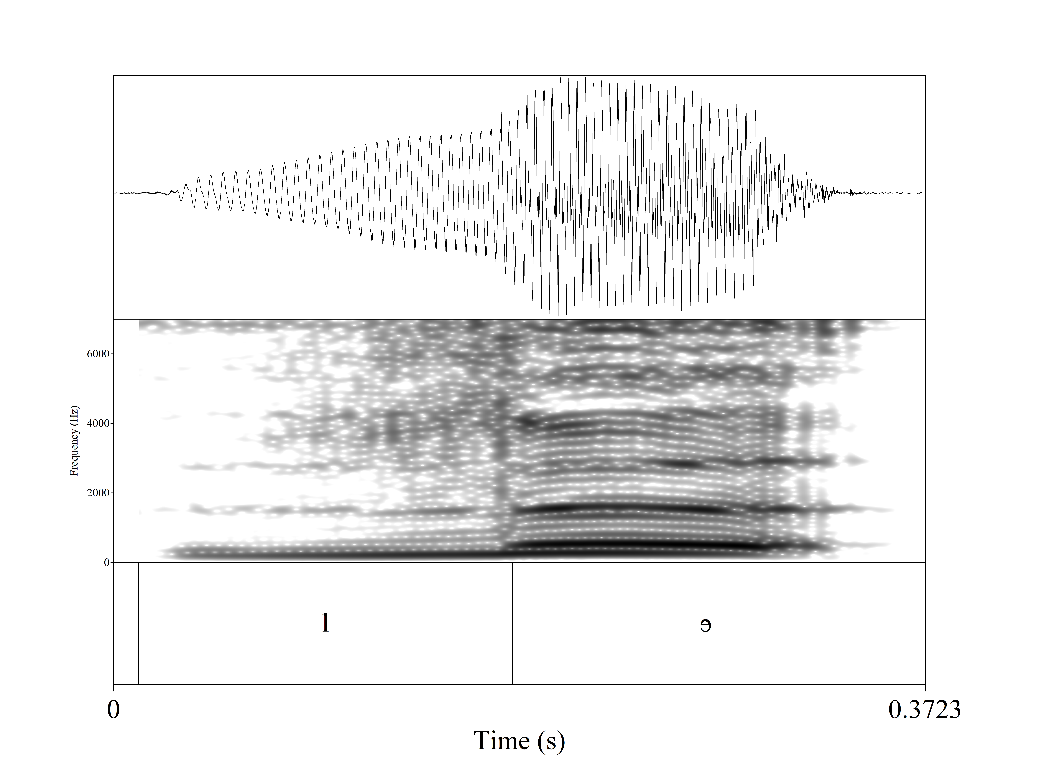
\includegraphics[height=.45\textheight]{figures/Guan-img002.png}
\caption{Spectrogram for lɘ́ ‘seed’} 
\label{fig:guan:2}
\end{figure}

\begin{figure}
\caption{Spectrogram for \textit{lɘ́ʶ} ‘highland wheat’}
\label{fig:guan:3}
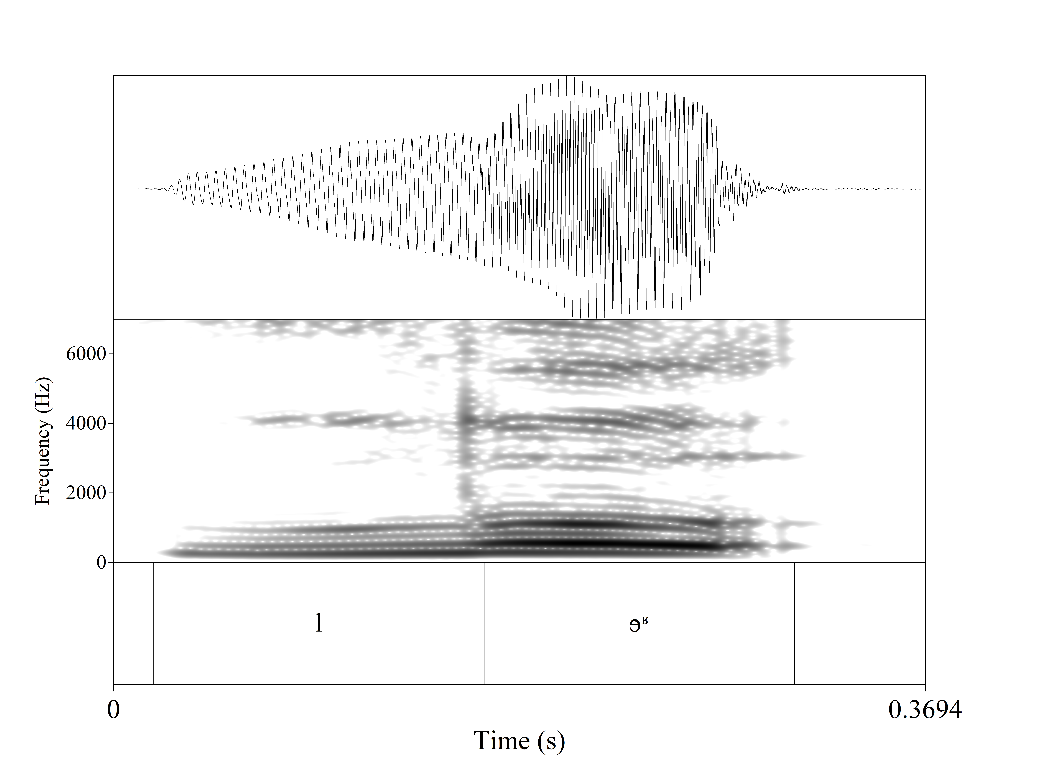
\includegraphics[height=.45\textheight]{figures/Guan-img003.png}
\end{figure}

Phonologically speaking, uvularized vowels trigger uvular allophones of preceding velar consonants. Uvular consonants occur before uvularized vowels only, and velar consonants only occur before plain vowels. This complementary distribution of dorsal consonants is best demonstrated in the allomorphic alternation of the verbal prefixes \textit{kɘ-} and \textit{qɘʶ-}, discussed in \sectref{sec:guan:2.3.3}.

There is one diphthong, /eɪ/, that is attested only in Tibetan loanwords thus far (e.g. \textit{hméɪ} ‘medicine’). Other potential diphthongs, such as [ye, ui, uə, uɑʶ, ie, iæ, iɑʶ] have been analyzed and transcribed here as the consonant\hyp vowel sequences /ɥe, wi, wə, wɑʶ, je, jæ, jɑʶ/, respectively. The glide /w/ has an allophone [ɥ], conditioned by the frontness of the following vowel and/or the place of articualtion of the preceding consonant. The phonemes /ʏ/ and /iʶ/ each occur only once in my data, in \textit{nʏ̌{} } ‘rest.3’, and \textit{xsʰí{} ʶ} ‘see clearly’. The latter word reflects the Written Tibetan \textit{gzhigs}\footnote{In this chapter I use Wylie's transcription for Written Tibetan \citep{Wylie1959}.} ‘to see’. 

  Queyu is a tonal language. Two tones are distinguished on monosyllabic words, a high level tone (e.g. ǽ) and a rising tone (e.g. æ̌). The high level tone on monosyllabic words can also be pronounced as a high falling tone without changing the meaning. When it comes to multisyllabic words, a low level tone may occur (e.g. æ̀). But a word can never bear only low level tone. For example, for disyllabic words, three tonal patterns are observed: high + high, high + low, low + high. The combination of low + low or a monosyllabic word bearing only low tone are never found in the data. 
In multisyllabic words and connected speech, the rising tone can sometimes be realized as a low level tone or high level tone. For example, the egophoric marker \textit{tsɨ̌} ‘\textsc{ego}’ and the generic marker \textit{tʂɨ̌} ‘\textsc{gnr}’ bear a rising tone when pronounced in isolation. When the two words are pronounced together, the tone pattern becomes low level + high level: \textit{tsɨ̀ tʂɨ́} ‘something that happens on a regular basis / it is the case that…’. Two consecutive rising tones within a word are not found in the present data set, either. When combining two morphemes with a rising tone, one or both morphemes’ tones will change. Below are examples demonstrating contrastive tones in monosyllabic words, tonal patterns in disyllabic words, and tonal change in morphosyntactic processes. For more details on the description and analysis of tones, plase refer to \citet{Guan2024}.
xlǐ
\ea%1
    \label{ex:guan:1}
    \ea Monosyllabic words\label{ex:guan:1a}
        \ea High level      \textit{xlí}  ‘tongue’
        \ex Rising      \textit{xlǐ{} }  ‘rabbit’
        \z
    \ex\ Disyllabic words \label{ex:guan:1b}
        \ea high + high    \textit{kʰímí}  ‘bovine’
            \ex high + rising    \textit{l̥ʊ́ʶbə̀{} }  ‘wind’
            \ex rising+ high    \textit{tʂʊ̀mbɘ́}‘justice’
        \z
    \ex\ Combination of morphemes \label{ex:guan:1c}
        \ea Rising      \textit{tə̌-{} }  ‘\textsc{pfv}’
             \ex Rising              \textit{kʰʊ̌{} }  ‘give.1\textsc{sg}’
             \ex
             \gll \textit{ŋə̌{} tə̀-kʰʊ́}\\
             1\textsc{sg} \textsc{pfv}-give.1\textsc{sg} \\
             \glt ‘I gave.’
        \z
    \z
\z

\subsubsection{Queyu syllable structure}\label{sec:guan:2.2.2}
The syllable structure of Queyu isː (P) (C) (G) V. A preinitial (P) is the first consonant of two non-glide consonants in the onset. Their intensity and duration are much shorter than those of regular consonants. The consonants (including allophones) that can appear in the preinitial position are limited to twelve: [p, b, ɸ, β, x, ɣ, χ, h, n, m, ŋ, ɴ]. Their distribution is partly predictable. Properties such as voicing and manner of a preinitial can be conditioned by the following consonant. For example, [p] occurs before voiceless coronal consonants, while [b] occurs before voiced stops and fricatives. [ɸ] occurs only before lateral sounds, and [β] occurs before voiced fricatives and liquids. C stands for any consonant, and G represents a glide. Three consonants can fill the glide slot. These are [j, w, ɥ], with [ɥ] being an allophone of /w/ conditioned by the following front vowel or preceding velar consonant. More information on the phonotactics of Queyu can be found in \citet{Guan2024}. Below are illustrative examples of each onset combination.
\ea%2
    \label{ex:guan:2}
\begin{xlist}
\item V    \textit{í{} {}-}  ‘\textsc{up}’
\item CV   \textit{və́}  ‘flour, powder’ 
\item GV    \textit{jæ̌-}  ‘\textsc{up.q}’
\item PCV  \textit{xpʰí}  ‘dust, ash’
\item CGV  \textit{vjé}  ‘pig’ 
\item PCGV  \textit{xpjé}  ‘rough, coarse’
\end{xlist}
\z
\subsection{The spreading of uvularization and other features in Pubarong Queyu prefixes}\label{sec:guan:2.3}

Uvularization in Pubarong Queyu can spread leftward across a morpheme boundary within a word. This is most clearly seen in the alternation of two sets of verbal prefixes, plain and uvularized. 

One way to analyze the alternation of prefixes is through the lens of vowel harmony. Though not common in TB languages, vowel harmony is consistently reported in Qiangic and Naic languages within the TB family (\citealt{Chirkova2024}ː 1). However, some Queyu data presents patterns that do not fit the traditional definition of vowel harmony, as is examined in more detail in \sectref{sec:guan:2.3.3}.

This section presents data on the spreading of uvularity and other features in Queyu prefixes. A brief typological overview on vowel harmony as well as an examination of argument indexation on verbs will be presented first in Sections \ref{sec:guan:2.3.1} and \sectref{sec:guan:2.3.2}. Information given in these sections will serve as a background for demonstrating and discussing how allomorphs of prefixes are conditioned in \sectref{sec:guan:2.3.3}.

\subsubsection{A brief overview of vowel harmony and uvulars in the Eurasian context}\label{sec:guan:2.3.1}


Traditionally speaking, vowel harmony refers to the agreement among all vowels in a word (or the harmonic domain) for some feature \citep{Hulst2016}. Vowel harmony patterns can vary based on different parameters, including static vs. dynamic harmony, root-controlled vs. dominant-recessive harmony, and directionality \citep{Makeeva_and_Kuznetsova_2022}. In terms of static vs. dynamic harmony, Pubarong Queyu uvularized vowels in verbs can trigger the appearance of uvularized verbal prefixes, indicating that Queyu belongs to the dynamic harmony type. As for the second and the third parameters mentioned above, vowels in the verbal prefixes are subject to harmony, while suffix vowels are not, indicating that Queyu data demonstrate regressive root-controlled harmony. In addition to the vowels in the verb stem, a voiced velar preinitial in the verb can also trigger a uvularized prefix, which is not commonly seen in vowel harmony cases. Furthermore, this feature spreading can affect the onset consonant of the prefix, which is also not typical for vowel harmony. Lastly, three verbal prefixes are not subject to this harmony process, despite the fact that the hypothetical uvularized versions of them are phonetically and phonologically possible in Queyu, while two vowels, /u/ and /o/, behave like plain vowels in some verbs and uvularized vowels in other verbs.  

Geographically speaking, vowel harmony is a major areal feature in Eurasian languages spoken in Northeast Asia (\citealt{BarrereJanhunen2019}ː 47). There are two major types of vowel harmony systems in languages spoken in Eurasia: palatal-velar harmony (PVH) and tongue root harmony\footnote{TRH is also prevalent in African languages, but these are not discussed here.}  (TRH) (\citealt{BarrereJanhunen2019}: 47). Palatal-velar harmony distinguishes palatal (front) and velar (back) vowels and is prevalent in languages spoken in the western part of Eurasia, while tongue root harmony distinguishes vowels with advanced vs. retracted tongue root (ATR/RTR) and is prevalent in languages spoken in the eastern part of Eurasia. The Mongolic family is in a transitional state with both types of harmony systems (\citealt{BarrereJanhunen2019}: 47--48). There is controversy regarding which type is more archaic, with some studies arguing for the greater antiquity of TRH (\citealt{Ko2012}, \citealt{KoEtAl2014}) and other studies arguing that TRH is merely an ancient areal feature introduced from the Northeast Pacific Rim (\citealt{BarrereJanhunen2019}). TRH presents a type of harmony comparable with that present in Queyu and other Qiangic languages.

The presence of uvular consonants in Southwest China is also considered to be an areal feature. \citet[124]{Hill2019} describes the region as a “uvular-prone Sprachbund” and considers the presence of uvular sounds in local Tibetan and Mongolian languages to reflect the influence of a Qiangic substrate. Similarly, post-velar consonants are commonly reported as phonemes or allophones of velar consonants in Mongolic and other Northeast Asian languages (\citealt{Nugteren2011}: 30--33, \citealt{Sylak-Glassman2014}: 32--36). The phonological phenomenon of vowel harmony related to post-velar consonants is also one of the major areal features of languages spoken in that region (\citealt{BarrereJanhunen2019}: 47, \citealt{Robbeets2020}: 129). A study investigating the geographical patterning of ejectives and uvulars suggests that language contact plays an important role in the development of uvular sounds in TB languages (\citealt{UrbanMoran2021}ː 27).

\subsubsection{Argument indexation on Queyu verbs}\label{sec:guan:2.3.2}


Pubarong Queyu presents complex argument indexation patterns. While argument indexes are suffixed to verb stems, they fuse with the vowel in the verb stem but do not effect change in the stem vowel quality. Vowel fusion processes are prevalent in Pubarong Queyu but will not be examined in detail in this chapter. All verbs contain a stem vowel, and when the stem is fused with a person suffix, the fused vowel is considered as part of the stem. Except for the situations illustrated in Sections \ref{sec:guan:2.3.3} and \ref{sec:guan:2.4}, the fused vowel can condition the prefix allomorph. This subsection merely provides a basic description of the verb types and argument suffixes to lay the groundwork for discussing allomorphic alternation in verbal prefixes in \sectref{sec:guan:2.3.3}.

There are three types of verbs based on the conjugation patterns. The first type does not conjugate for person or number. A large class of this type is stative verbs, or verbs expressing property concepts. Several examples of this type include ‘big’ \textit{ndʒʉ́ʶ}, ‘say, speak’ \textit{pʃə́}, ‘win, beat’ \textit{kʰǐ}, ‘lock (a door)’ \textit{kwə́}, and ‘dig’ \textit{pɘ́ʶqwə́ʶ}. 

The second type of verb only distinguishes Speech Act Participants (SAP) and non SAP, with the non SAP form containing an inserted bilabial consonant—a relic of an inverse marker still prevalent in nearby Rgyalrongic languages. Examples of this type include ‘throw’ (\textit{ɽə́} for SAP form and \textit{βɽə́} for non-SAP form), ‘pay, submit’ (SAP formː \textit{ɖɽæ̌}, non-SAP formː \textit{ɖɽwæ̌}), ‘cut, saw’ (SAP formː \textit{ʈɽæ̌}, non-SAP formː \textit{pʈɽæ̌}), ‘wipe’ (SAP formː \textit{də́}, non-SAP formː \textit{bdə́}), ‘release’ (SAP formː \textit{l̥ə́ʶ}, non-SAP formː \textit{ɸl̥ə́ʶ}), and ‘hand, give’ (SAP formː \textit{xtə́ʶ}, non-SAP formː \textit{xtwə́}). 

The third type of verb contrasts both person and number. This is the type that shows the most diversity. Within this type, first person singular and plural forms end with \textit{{}-ʊ} and \textit{{}-æ} for plain vowel stems (such as ‘say, speak’ and ‘feed, give’ in \tabref{tab:guan:4}), and with {}-\textit{ʊʶ} and \textit{{}-aʶ} for uvularized vowel stems, respectively. Only a few verbs with a plain vowel stem contrast number in second person (such as ‘say, speak’), while verbs with uvularized vowels do not distinguish number in second person. Third person forms exhibit the greatest variation. Some third person forms contain an inserted bilabial consonant like the second type of verb described above (e.g. ‘sit’, ‘dip’, ‘hold, take’), while others do not (e.g. ‘say, speak’, ‘feed, give’, ‘poke, stab’). Several examples of this type are demonstrated below.

\begin{table}
\caption{Verbs that contrast both person and number}
\label{tab:guan:4}
\begin{tabularx}{\textwidth}{XXXXXl}
\lsptoprule
{Verb} & {1\textsc{sg}} & {1\textsc{pl}} & {2\textsc{sg}} & {2\textsc{pl}} & {3}\\
\midrule
{‘say, speak’} & {ɲʊ̌} & {ɲ\v{æ}} & {nɘ̌} & {ɲɪ̌} & {ɲǐ}\\
{‘feed, give’} & {ʃ\v{ʊ}} & {ʃ\v{æ}} & {ʃ\v{ɨ}} & {ʃ\v{ɪ}} & {ʃ\v{y}}\\
{‘sit’} & {tsʊ́} & {ts\'{æ}} & {tsɪ́} & {tsɪ́} & {ptsʊ́}\\
{‘dip’} & {ʃə́ʶʃʊ́ʶ} & {ʃə́ʶʃɑ́ʶ} & {ʃə́ʶʃéʶ} & {ʃə́ʶʃéʶ} & {ʃə́ʶpʃʊ́ʶ}\\
{‘hold, take’} & {z\v{ʊ}ʶ} & {z\v{ɑ}ʶ} & {z\v{e}ʶ} & {z\v{e}ʶ} & {βz\v{ʊ}ʶ}\\
{‘poke, stab’} & {xtʃʰ\v{ʊ}ʶ} & {xtʃʰ\v{ɑ}ʶ} & {xtʃʰ\v{e}ʶ} & {xtʃʰ\v{e}ʶ} & {xtʃʰ\v{ʉ}ʶ}\\
\lspbottomrule
\end{tabularx}
\end{table}

\subsubsection{Allomorphic alternations of verbal prefixes}\label{sec:guan:2.3.3}


Uvularization in Pubarong Queyu can spread leftward across morpheme boundaries. This is most clearly seen in the verbal prefixes that are given in \tabref{tab:guan:7} in comparison to the prefixed verb examples in \tabref{tab:guan:6}. For most prefixes, there are two sets which can be conditioned by the vowel quality in the verb stem. Only the prefixes for ‘downstream’ and the three allomorphs for ‘upward’ do not have uvularized forms. \tabref{tab:guan:5} illustrates the plain and uvularized versions of the prefixes, which include six directional prefixes (prefixes that indicate the direction of motion), a question marker, a prohibitive marker, and three negation prefixes that are used in different TAME contexts. Among them, only two directional prefixes and a negation prefix do not have uvularized forms, and they are the ‘downstream’ and the three allomorphs for ‘upward’ prefixes, as well as the méɪ- negation marker.

\begin{table}
\caption{Prefixes in Queyu}
\label{tab:guan:5}
\begin{tabularx}{\textwidth}{XXl}
\lsptoprule
{Queyu prefix} & {Uvularized version} & {Gloss}\\
\midrule
{í-, rɨ́, ɘ́-} & {{}-}  & \textsc{up}\\
{n\v{ə}-} & {n\v{ə}ʶ-} & \textsc{down}\\
{lə́} & {lə́ʶ-} & \textsc{upstream}\\
{\v{i}-} & {{}-}  & \textsc{downstream}\\
{kɘ́-} & {qɘ́ʶ-} & \textsc{in}\\
{t\v{ə}-} & {t\v{ə}ʶ-} & {\scshape pfv}\\
{\`{æ}-} & {ɑʶ-} & {\scshape q}\\
{t\'{æ}-} & {tɑʶ-} & {\scshape proh}\\
{m\'{æ}-} & {mɑʶ-} & {\scshape neg}\\
{m{ə}-} & {məʶ-} & {\scshape neg}\\
{m\'{e}ɪ-} & {-} & {\scshape neg}\\
\lspbottomrule
\end{tabularx}
\end{table}


\tabref{tab:guan:6} presents examples of prefixed verbs with plain vowel argument suffixes. Notice that the directional prefixes can also function as perfective and imperative markers in addition to indicating the direction of motion. When this is the case, the change in meaning is explained in the translation according to the context.

\vfill
\begin{table}[H]
\caption{Prefixes with verbs containing plain vowel suffixes}
\label{tab:guan:6}
\begin{tabularx}{\textwidth}{XXl}
\lsptoprule
{Queyu} & {Gloss} & {Translation}\\
\midrule
{í-tʃì} & {\textsc{up}{}-go.3} & {‘go upwards’}\\
{nə̀-tʃí} & {\textsc{down}{}-go.3} & {‘go downwards’}\\
{lə́-tʃì} & {\textsc{upstream}{}-go.3} & {‘go upstream’}\\
{ì-tʃí} & {\textsc{downstream}{}-go.3} & {‘go downstream’}\\
{kɘ́-pə̀} & {\textsc{in}{}-wet} & {‘got wet’}\\
{tə̀-kʰwɪ́} & {\textsc{pfv}{}-give.3} & {‘He/she/it gave.’}\\
{\'{æ}-ʒí} & {\textsc{q}{}-delicious} & {‘Is it tasty?’}\\
{t\'{æ}-pʰɘ̀tʰɪ̀} & {\textsc{proh}{}-scatter.2} & {‘Don’t scatter!’}\\
{m\'{æ}-sʰí} & {\textsc{neg}{}-die} & {‘won’t die’}\\
{k\'{ə}-m\'{ə}-ɲʊ̀} & {\textsc{in}-\textsc{neg}{}-listen.1\textsc{sg}} & {‘I didn’t listen.’}\\
{m\'{e}ɪ-ndʊ̀} & {\textsc{neg}{}-see.1\textsc{sg}} & {‘I didn’t see it.’}\\
\lspbottomrule
\end{tabularx}
\end{table}
\vfill\pagebreak


Uvularized prefixes can be triggered by the vowel quality of the vowel in the argument suffix. In \tabref{tab:guan:7}, examples of prefixes with verbs containing a uvularized vowel are presented. From the examples below, we see that the vowels in the prefixes are uvularized (except for the three situations mentioned above).

\begin{table}
\caption{Prefixes with verbs containing uvularized vowels}
\label{tab:guan:7}
\begin{tabularx}{\textwidth}{Xll}
\lsptoprule
{Queyu} & {Gloss} & {Translation}\\
\midrule
{í-zʊ̀ʶ} & {\textsc{up}{}-take away.1\textsc{sg}} & {‘I took’} \\
{nə̀ʶ-χqʊ́ʶ} & {\textsc{down}{}-boil.1\textsc{sg}} & {‘I boiled’}\\
{lə́ʶ-xpʰə̀ʶ} & {\textsc{upstream}{}-vomit} & {‘(someone) threw up’}\\
{ì-xtʊ́ʶ} & {\textsc{downstream}{}-closed (door).1\textsc{sg}} & {‘I closed the door.’}\\
{qɘ́ʶ-pə̀ʶ} & {\textsc{in}{}-rot} & {‘(It is) rotten.’}\\
{tə̀ʶ-hmʊ́ʶ} & {\textsc{pfv}{}-close (eyes).1\textsc{sg}} & {‘I closed (eyes).’}\\
{ɑ́ʶ-xsʰíʶ} & {\textsc{q}{}-see clearly} & {‘Can you see clearly?’}\\
{jɑ́ʶ-zèʶ} & {\textsc{proh.downstream}{}-take.2} & {‘Don’t take it!’}\\
{mɑ́ʶ-xsʰíʶ} & {\textsc{neg}{}-see clearly} & {‘can’t see it clearly’}\\
{nɘ́ʶ-mɘ́ʶ-χqò} & {\textsc{down}{}-\textsc{neg}{}-trouble} & {‘You are welcome.’}\\
{méɪ-mə̀ʶ} & {\textsc{neg}{}-hear} & {‘I didn’t hear it.’}\\
\lspbottomrule
\end{tabularx}
\end{table}


Beyond the vowel, it is worth noting that for the ‘inward’ prefix \textit{kɘ́-}, the plain form has a velar initial consonant. When the verb stem contains a uvularized vowel, uvularity not only spreads to the vowel in the prefix, but also to the initial stop, change it to a uvular, hence the form \textit{qə́ʶ}{}-. Examples ‘got wet’ \textit{kɘ́-pə̀ {} } from \tabref{tab:guan:6} and ‘rotten’ \textit{qɘ́ʶ-pə\`{} ʶ} from \tabref{tab:guan:7} illustrate this alternation. This alternation is the reason I term this phenomenon in Queyu “uvularization” instead of “velarization” or “pharyngealization”. In addition, this allomorphic alternation is one piece of evidence that Queyu data do not present a typical case of vowel harmony, as consonants also undergo uvularization.

Uvularization does not spread rightwards, as suffixes containing plain vowels remain plain when following a stem that contains uvularized vowels. Examples with a plain vs. uvularized root are given in \REF{ex:guan:3} and \REF{ex:guan:4}. The patient nominalizer \textit{{}-ʃə{} } contains a plain vowel, regardless of the vowel quality in the preceding root.

\ea%3
    \label{ex:guan:3}
    \gll  tʃʰɨ́-ʃə̀{} \\
  eat-\textsc{nmlz}\\
\glt   ‘food’
    \z

\ea%4
    \label{ex:guan:4}
    \gll    ptə̀ʶ-ʃə́{} \\
  chop-\textsc{nmlz}\\
\glt   ‘things to be chopped’
    \z

Uvularized prefixes can also be triggered when the stem contains a voiced velar preinitial, which is demonstrated in examples \xxref{ex:guan:5}{ex:guan:7}. The vowels in verb stems are plain in \xxref{ex:guan:5}{ex:guan:7}, but these verbs still pair with uvularized prefixes. The only thing these verbs share in common is that they contain a voiced velar preinitial. The fact that uvularized prefixes can be conditioned by consonants, in the absence of a uvularized vowel, is further evidence indicating that uvularity spreading in Pubarong Queyu may not be vowel harmony in the classical sense.

\ea%5
    \label{ex:guan:5}
    \gll nə̀ʶ{}-ɣɲʊ́\\
  \textsc{pfv}-knead.1\textsc{sg}\\
\glt   ‘I kneaded (the dough).’
    \z

\ea%6
    \label{ex:guan:6}
    \gll tə̀ʶ{}-ɣʒʊ́\\
  \textsc{pfv}-toss.1\textsc{sg}\\
 \glt   ‘I tossed (something).’    \z

\ea%7
    \label{ex:guan:7}
    \gll ʃʰʊ̀pʃʰí  qɘ́ʶ-ɣʒɥè\\
  child \textsc{pfv}-feed\\
\glt   ‘I raised (provide food and materials for) kids.’
    \z

There is another type of vowel alternation in verbal prefixes unrelated to uvularization. See \REF{ex:guan:8} and \REF{ex:guan:9}, where the directional prefixes \textit{lə́-} turns into \textit{lɘ́-} when followed by \textit{mɘ-} and \textit{tæ-}, and \textit{nə̌-} into \textit{nɘ̌-} when followed by \textit{tæ-}. This type of alternation differs from those just described. The verb stem vowel does not seem to play a role in conditioning the prefixes, as can be seen in the comparison between \REF{ex:guan:8a} and \REF{ex:guan:8b}. The verb stem vowel remains the same, but the vowel in the directional prefix changes. However, as uvularity spreading is root controlled, meaning the feature in the verb stem determins the prefix vowel quality, the changed prefixes can still have a uvularized counterpart. This is demonstrated in \REF{ex:guan:10} and \REF{ex:guan:11}, where the uvularized \textit{lɘ́ʶ-}, \textit{mɘʶ-}, and \textit{taʶ-} occur. For this type of vowel change, with only limited examples so far, no concrete conclusion can be drawn. More data are needed for further exploration of this type of prefix alternation. 

\ea%8
The \textit{lə́-} prefix changes to \textit{lɘ-} when preceding \textit{mɘ-} and \textit{tæ-}:
    \label{ex:guan:8}
    \ea \label{ex:guan:8a}
        \gll lə́-ʃʰʊ̀\\
        \textsc{upstream}{}-go.1\textsc{sg}\\
        \glt  ‘I went upstream.’
    \ex \label{ex:guan:8b}
        \gll lɘ́-mɘ́-ʃʰʊ̀\\
        \textsc{upstream}{}-go-\textsc{neg}.1\textsc{sg}\\
        \glt  ‘I didn’t go upstream.’
    \ex \label{ex:guan:8c}
        \gll lɘ́-tæ̀-ʃʰɨ̀\\
        \textsc{upstream}-\textsc{proh}-go.2\textsc{sg}\\
        \glt  ‘Don’t go upstream.’
        \z
    \z
        
\ea%9
The \textit{nə̌-} prefix changes to \textit{nɘ-} when preceding \textit{tæ-}:
    \label{ex:guan:9}
    \ea \label{ex:guan:9a}
        \gll nə̀-ʃʰʊ́\\
        \textsc{down}{}-go.1\textsc{sg}\\
        \glt  ‘I went down (to Chengdu’s direction).’
    \ex \label{ex:guan:9b}
        \gll nɘ́-tæ̀-ʃʰɨ\\
        \textsc{down}-\textsc{proh}-go.2\textsc{sg}\\
        \glt  ‘Don’t go (to Chengdu’s direction).’
        \z
        \z

\ea%10
The \textit{lɘ́ʶ-} and \textit{mɘʶ-} prefixes can also be uvulairzed: 
    \label{ex:guan:10}
    \ea \label{ex:guan:10a}
        \gll lə́ʶ-xpʰə̀ʶ\\
        \textsc{upstream}{}-vomit\\
        \glt  ‘(Someone) vomited.’        
    \ex \label{ex:guan:10b}
        \gll nɘ́-tæ̀-ʃʰɨ\\
        \textsc{upstream}-\textsc{neg}-vomit\\
        \glt  ‘(Someone) hasn’t vomited yet.’
        \z
    \z
        
\ea%11
The prohibitive marker \textit{taʶ-} can also be uvularized:
    \label{ex:guan:11}
    \ea \label{ex:guan:11a}
        \gll ɘ́-zèʶ\\
        \textsc{up}{}-take.2\\
        \glt  ‘(You) take it.’
    \ex \label{ex:guan:11b}
        \gll í-tàʶ-zèʶ\\
        \textsc{up}-\textsc{proh}-take.2\\
        \glt  ‘Don’t take it.’
        \z
    \z
        

\subsection{Exceptions to vowel harmony}\label{sec:guan:2.4}\largerpage

While plain and uvularized vowels in a verb stem can trigger different sets of prefixes, there are two vowels that do not follow this patternː /o/ and /u/. Some verbs containing these two vowel suffixes pair with plain prefixes, while others trigger a uvularized allomorph. As shown in \tabref{tab:guan:8}, verbs containing /o/ and \mbox{/u/} can pair with uvularized prefixes. Morphologically speaking, the /o/ and /u/ phonemes in these cases trigger uvularized prefixes, which is strong evidence suggesting that /o/ and /u/ belong to the uvularized set of vowels.

\begin{table}
\caption{Vowels /o/ and /u/ exhibiting uvularized vowel behavior}
\label{tab:guan:8}
\begin{tabularx}{\textwidth}{XXl}
\lsptoprule
{Lexicon} & {Gloss} & {Translation}\\
\midrule
{qɘ́ʶ-dò } & {\textsc{in}{}-tie} & {‘tied up, chained up’}\\
{ɑ́ʶ-tʂó} & {\textsc{q}{}-cold} & {‘Is it cold?’}\\
{tɑ̌ʶ-xtù} & {\textsc{pfv.q}{}-hit.3} & {‘Did he hit?’}\\
\lspbottomrule
\end{tabularx}
\end{table}


However, in some verbs /o/ and /u/ behave like plain vowels. From \tabref{tab:guan:9}, we see that ‘happy’ \textit{ɡó}, ‘dance’ \textit{dʒó,} and ‘hug’ \textit{xtú} pair with a plain prefix. If /o/ and /u/ were behaving like uvularized vowels in these words, they would trigger the uvular allomorphs of the prefixes. Additionally, if uvular consonants in Pubarong Queyu are allophones of velar sounds triggered by uvularized vowels, then the fact that ‘happy’ \textit{ɡó} starts with a velar consonant rather than a uvular consonant suggests that /o/ behaves like plain vowel here.

\begin{table}
\caption{Vowels /o/ and /u/ exhibiting plain vowel behavior}
\label{tab:guan:9}
\begin{tabularx}{\textwidth}{XXl}
\lsptoprule
{Lexicon} & {Gloss} & {Translation}\\
\midrule
{m\'{æ}{}-ɡó} & {\textsc{neg}{}-be.happy} & {‘unhappy’}\\
{m\'{æ}{}-dʒó} & {\textsc{neg}{}-dance} & {‘won’t dance’}\\
{j\v{æ}-xtù} & {\textsc{pfv.q}{}-hug.3} & {‘Did he hug?’} \\
\lspbottomrule
\end{tabularx}
\end{table}

Another piece of morphological evidence suggesting that /u/ behaves both as a plain and a uvularized vowel comes from verbal paradigms. There are both plain and uvularized verbs whose third person forms end with a \textit{{}-u} suffix. Examples are given below.

\begin{table}
\caption{3rd person verb forms ending with /u/}
\label{tab:guan:10}
\begin{tabularx}{\textwidth}{lXXXXl}
\lsptoprule
{Gloss} & {1\textsc{sg}} & {1\textsc{pl}} & {2\textsc{sg}} & {2\textsc{pl}} & {3}\\
\midrule
{‘buy’} & {xkʊ́} & {xkǽ} & {xkɪ́} & {xkɪ́} & {xkú}\\
{‘hit, pound'} & {xtʊ̌ʶ} & {xtɑ̌ʶ} & {xtɪ̌ʶ} & {xtɪ̌ʶ} & {xtǔ}\\
\lspbottomrule
\end{tabularx}
\end{table}


Since /o/ and /u/ may behave like either plain vowels \textit{or} uvularized vowels, this is further evidence that analyzing this data from a traditional vowel harmony perspective can be problematic. That /o/ and /u/ behave like both plain and uvularized vowels suggests that historically for each there may have been be two sets of vowels, plain and uvularized, that have merged into /o/ and /u/ respectively.\footnote{Personal communication with Dr. Lin You-jing and Dr. Lai Yunfan.} Phonetically there is no distinction now, and there is only morphophonological evidence as a trace of this possible merger.\footnote{However, we cannot rule out the hypothesis that /oʶ/ and /uʶ/ still exist. Further acoustic measurements are required to investigate this issue. I would like to thank Dr. Spike Gildea for pointing this out.}

\section{Uvularized vowels and other similar vowels in regional typological studies}\label{sec:guan:3}

The data presented above show that Queyu contrasts plain and uvularized vowels. Uvularity in Queyu can spread leftward across morpheme boundaries, which is best evidenced by the presence of uvularized prefixes triggered by uvularized vowels in verbs. In addition to vowels, velar consonants can also be the target of uvularization, as they become uvular consonants when preceding a uvularized vowel. Uvularized prefixes can also be triggered by a voiced velar preinitial consonant in the verb stem. Two vowels, /o/ and /u/, do not follow this pattern, and behave as plain \textit{and} uvularized both morphosyntactically and morphophonologically. The vowel /o/ can occur after both non-uvular and uvular consonants, and \textit{{}-u} can be a verbal suffix for third person forms in both paradigms, pairing with both plain and uvularized prefixes.

These facts lead to the following four questionsː 

\begin{enumerate}
\item What are the phonetic differences between plain and uvularized vowels in terms of acoustics and articulation? 
\item How can we account for the spreading of uvularity in Pubarong Queyu?
\item What is the origin of the uvularized vowels in Pubarong Queyu? 
\item For /u/ and /o/, one possible hypothesis is that there used to be both /u/ and /uʶ/, and /o/ and /oʶ/ which then merged into /u/ and /o/ respectively. Or could /uʶ/ and /oʶ/ still exist in this language? 
\end{enumerate}

This section presents data from closely-related languages attesting similar phenomena, and aims to address the first three questions. Literature on other Qiangic languages are introduced first, and it is important to note that different terms have been used to label marked vowel qualities, similar to Queyu’s uvularized vowels, in Qiangic/Rgyalrongic languages. There is no consensus among Tibeto-Burmanists about how to describe and analyze the phenomena associated with uvularization and other similar vowel qualities. Detailed comparison among each author’s suggestions will be beyond the scope of this chapter; therefore readers are suggested to consult the original works mentioned here for further reference. \sectref{sec:guan:3} merely presents a summary of the current available literature on this topic within Qiangic/Rgyalrongic. Tables and data from other languages in this section are reproduced from other works with no changes made to transcription or glossing style.

  This overview of the literature has two aims. The first is to introduce the current state of the analysis of uvularization and relevant phenomena within Qiangic/Rgyalrongic. The second is to show discrepancies in current findings on this topic that have not been well explained and draw attention to the need for more acoustic studies and systematic explanations. 

In this section, a brief summary of uvularized vowels and similar vowel qualities in the TB family is given in \sectref{sec:guan:3.1}, followed by an examination of the articulation of uvularized, velarized, and pharyngealized vowels in \sectref{sec:guan:3.2}. \sectref{sec:guan:3.3} reviews acoustic and ultrasound studies done in Qiangic/Rgyalrongic languages, summarizing the acoustic characteristics of the marked vowels in comparison with their plain counterparts. \sectref{sec:guan:3.4} presents information on vowel harmony within Qiangic, a phenomenon associated with uvularization. \sectref{sec:guan:3.5} discusses possible origins of phenomena relevant to uvularization.

\subsection{Similarities among uvularized, velarized, and pharyngealized vowels noted in the literature}\label{sec:guan:3.1}

While velarization and pharyngealization are usually secondary articulations associated with consonants, these qualities are vowel features in Qiangic languages such as Puxi Stau (\citealt{LadefogedMaddieson1996}: 360, 365, \citealt{LinEtAl2012}: 87). The similarity between velarization and pharyngealization is noted in \citet[236]{LadefogedJohnson2011}, who point out that there is no language that distinguishes these two possibilities. This similarity is also brought up several times in the descriptions of Qiangic languages summarized below.

The rare vowel distinction discussed here is first mentioned for a TB language in \citegen{Sun2000b} description of verbal inflection in the Puxi variety of Stau, under the term “velarization”. \citet{Evans2006a,Evans2006b} describes the vowel quality in the Hongyan variety of Northern Qiang as “pharyngealization” and discusses the feature’s origins. \citet{Evans2006b} is the first study that addresses pharyngealization in TB languages. Evans (\citeyear*{Evans2006a}: 94; \citeyear*{Evans2006b}: 737) mentions that Jackson Sun, through personal communication, has pointed out the phonetic similarity between velarized vowels in Rgyalrongic languages and pharyngealized vowels in Hongyan Qiang. In a later study, \citet{SunEvans2013} revisit the vowel quality issue in Yunlinsi (Hongyan) Qiang, and amend the analytical umbrella label to “uvularization” rather than “pharyngealization”.

In a study on uvularization in Tangut, an extinct Qiangic language, \citet[193--194]{Gong2020} reconstructs uvularized vowels, describing uvularization in Qiangic languages as a case of guttural secondary vocalic articulations (GSVA), and notes that this distinction is similar to one found in Eastern Minyag,\footnote{However, the literature that \citet{Gong2020} cited, i.e. \cite{Huang1985} and \citet{Gao2015}, are based on Minyag spoken in Kangding, which is classified as the Western variety of Minyag rather than  the Eastern variety. This chapter keeps the original wording of the source literature when citing them, but the mismatch in use of terminology should be noted.} which is described as a lax/tense distinction by \citet{Huang1985} and as an ATR/RTR (Advanced tongue root/Retracted tongue root) distinction by \citet{Gao2015}. In Eastern Minyag, velar consonants only occur preceding lax/ATR vowels, and uvular consonants only occur preceding tense/RTR vowels. The Eastern Minyag tense/RTR vowels, to Gong’s ear, sound as though they contain pharyngealization \citep[194]{Gong2020}.

Pharyngealized vowels are also found in non-Qiangic languages of the region. \citet{Suzuki2011} presents data on pharyngealized vowels in Gagatang Tibetan and examines their origins by comparing data from Written Tibetan, adjacent Tibetan varieties, and Naxi, a local Naic language. He discusses the connection between pharyngealization and rhotacization in vowels and points out in a later study \citep[29--31]{Suzuki2013} that rhotacized vowels in Naxi are velarized or pharyngealized in some varieties. He also notes that the tense vowels in Naxi brought up by \citet{Yang1984,Yang1991} correspond to rhotacized vowels in other scholars’ descriptions. It is worth noting that the pharyngealized vowels found in Gagatang Tibetan are unique among Tibetic varieties \citep[489]{Suzuki2011}. Furthermore, Gaga\-tang Tibetan is spoken in Yunnan Province, near the border of Sichuan Province, just to the south of where the Qiangic languages are spoken. The languages within the family attested to have these vowel distinctions are therefore spoken roughly within the same geographical region. \citet[492--493]{Suzuki2011} suggests that the development of pharyngealization in Gagatang Tibetan vowels may come from the influence of neighboring languages, possibly from Naxi. The spreading of uvular consonants is also suggested to be due to contact by \citet[27]{UrbanMoran2021} in Sino-Tibetan.

\subsection{The articulation of uvularized vowels and similar vowel qualities}\label{sec:guan:3.2}

\citet[235--236]{LadefogedJohnson2011} summarize that the back of the tongue is raised during velarization, and that pharyngealization involves the narrowing of the pharynx during articulation. Uvularized vowels are characterized by constriction of the styloglossus and other muscles, which draws the tongue dorsum towards the uvula (\citealt{EvansEtAl2016}: 1). Other vowel qualities such as velarization and pharyngealization mentioned in related languages have similar articulatory gestures. \citet[215]{Sun2000b} points out that the articulatory gestures of velarized vowels in Puxi Rgyalrong are characterized by the dorsum of the tongue arching towards velum. \citet{EvansEtAl2016} use ultrasound imaging to explore the articulatory gestures of uvularized vowels in Mawo and Luhua, two Northwestern Qiang varieties spoken in Heishui Town. In terms of articulation, ultrasound imaging shows that the tongue is retracted towards the uvular region when producing a uvularized vowel, in juxtaposition with a plain vowel counterpart (\citealt{EvansEtAl2016}ː 22). An ultrasound imaging study on pharyngealized vowels in two Northern Horpa (\textit{aka} Stau, Ergong, Daofu) varieties shows that the tongue body retracts and forms double bunching when producing pharyngealized vowels (\citealt{ChiuSun2020}ː 2938).

In sum, these articulations involve a stricture at the velum, uvula, or pharynx region, and the tongue body is usually retracted. The acoustic characteristics of these vowels are also similar, as will be addressed in \sectref{sec:guan:3.3}. The correlation between articulatory features and acoustic measurements will be discussed in the next subsection.

\subsection{Acoustic properties of uvularized, velarized, and pharyngealized vowels in Qiangic languages}\label{sec:guan:3.3}

There are occasional mentions of the similarities among uvularized, velarized, and pharyngealized vowel qualities in the literature on TB languages spoken in Southwest China. There are also mentions of the fact that these vowels can trigger vowel harmony. \citet[88]{LinEtAl2012} acoustically examine velarized vowels in Puxi Stau, finding that velarized vowels have a significantly lower F2 and a raised F3 when compared to their plain vowel counterparts. Though change in F1 is not significant, lower F2 indicates retraction of the tongue root, which matches the articulatory gesture identified for velarized vowels (\citealt{LinEtAl2012}: 88--89).

\citet{SunEvans2013} re-examine the vowel system in Mawo Qiang, a Northern Qiang variety with a series of uvularized vowels, finding the most prominent acoustic feature of uvularized vowels to be a lowered F2 (\citealt{SunEvans2013}: 141). Both F1 and F3 are raised in uvularized vowels as compared to their plain-vowel counterparts. 

\citet{EvansEtAl2016} also acoustically examine vowel uvularization in Mawo and Luhua Qiang. Compared to their plain counterparts, uvularized vowels have higher F1 (significant for non-schwa vowels), lower F2, and increased difference between F3 and F2. 

The study by \citet{Way2018} is a description and analysis of the phonetics and phonology of another Qiangic language, Nyagrong Minyag. He examines uvularization in vowels, and provides acoustic measurements which show a raised F1 value for uvularized high vowels compared to their plain counterparts ([i], [y], and [u]). He also finds a lower F2 for uvularized non-high vowels ([ə], [ɔ], and [a]). F3 is slightly increased in all uvularized vowels  except for [iʶ] and [aʶ] (\citealt{Way2018}ː 103). All in all, drop in F2 is found to be the most salient acoustic cue for uvularized vowels (\citealt{Way2018}ː 123). 

\citet{ChiuSun2020} examine pharyngealized vowels in two Northern Horpa (Stau) varieties—Rtsangkhog and Yunasche. In addition to the articulatory study mentioned in \sectref{sec:guan:3.2}, which found tongue retraction, backing, and double bunching during the production of pharyngealized vowels (\citealt{ChiuSun2020}: 2938), the authors conducted an acoustic study. The results showed that F1 is higher in pharyngealized vowels than in plain vowels and that this higher value corresponds to the lowering of the tongue (\citealt{ChiuSun2020}ː 2939). The change observed for F2 is not as consistent as that of F1, in that F2 is lowered substantially for most pharyngealized vowels, but not for [uˤ] in Rtsangkhog or [oˤ] and [uˤ] in Yunasche (\citealt{ChiuSun2020}ː 2941). For F3, the formant frequency increases for certain vowels ([əˤ], [ɐˤ], [oˤ] and [uˤ] in Rtsangkhog, [ɐˤ], [oˤ] and [uˤ] in Yunasche), and decreases for front vowels (\citealt{ChiuSun2020}ː 2941--2942).

\tabref{tab:guan:11} summarizes the results from previous studies on the comparison of formants between two sets of vowels (plain and uvularized/velarized/pharyngealized) in different Qiangic languages. Blank cells indicate that the study did not address a property specifically.

\begin{sidewaystable}
\footnotesize
\caption{Acoustic differences in Qiangic languages between uvularized/velarized/pharyngealized vowels and their plain counterparts. \emph{Note}: Although the acoustic measurements are inconsistent between plain and uvularized/velarized/pharyngealized vowels in the Rgyalrongic/Qiangic languages, this does not necessarily mean that vowel qualities/cues are different in different languages. Differences may emerge from insufficient statistical power, which is very likely in phonetics, especially with understudied languages, or between-speaker variability in cue use within the language. Another reason might be due to differences between methods of measurement or the design of experiments. Refinement of existing descriptions will need to test interactions between cues and the language. I would like to thank Dr. Volya Kapatsinski and Dr. Natalia Kuznetsova for bringing these points to attention.}
\label{tab:guan:11}
\tabcolsep=.66\tabcolsep
\begin{tabular}{lllllll}
\lsptoprule
Sources & {Language} & {Vowel quality} & {F1} & {F2} & {F3} & {F3-F2}\\
\midrule
\citet{LinEtAl2012} & {Puxi Stau} & {Velarization} & {No significant change} & {Decrease} & {Increase} & \\
\citet{SunEvans2013} & {Mawo Qiang} & {Uvularization} & {Increase} & {Decrease} & {Increase} & \\
\citet{EvansEtAl2016} & {Mawo Qiang} & {Uvularization} & Increase\footnote{significant for non-schwa vowels} & {Decrease} &  & {Increase}\\
& Luhua (Yunlinsi-Hongyan) & {Uvularization} & {Increase\textsuperscript{\textit{a}}} & {Decrease} &  & {Increase}\\
\citet{Way2018} & {Nyagrong Minyag} & {Uvularization} & {Increase}  & {Decrease} & {Increase\footnote{except for [iʶ] and [aʶ]}} & {Increase}\\
\citet{ChiuSun2020} & {Rtsangkhog Horpa} & {Pharyngealization} & {Increase} & {Decrease\footnote{except for [uˤ]}} & {Increase\footnote{significant for [əˤ], [ɐˤ], [oˤ] and [uˤ]}} & \\
& Yunasche Horpa & {Pharyngealization} & {Increase} & {Decrease\footnote{except for [uˤ] and [oˤ]}} & Increase\footnote{significant for [ɐˤ], [oˤ] and [uˤ]}, & \\
&                &                     &            &                                               & little difference\footnote{for [eˤ] and [əˤ]} & \\
\lspbottomrule
\end{tabular}
\end{sidewaystable}


\subsection{Vowel harmony in Qiangic}\label{sec:guan:3.4}

Despite the fact that different terms are used to describe vowel qualities in the Rgyalrongic/Qiangic languages reviewed in \sectref{sec:guan:3.1} and \sectref{sec:guan:3.2}, these vowel contrasts behave similarly in that they participate in a similar phonological process, vowel harmony. Vowel harmony is not common among TB languages, with most cases reported in Qiangic, and only a few in the Naic and Tibetic languages of the Himalayish subgroup \citep[729]{Chirkova2024}. \citet[10]{Sun2016} considers vowel harmony to be a feature of the Qiangic branch. While vowel harmony is commonly reported in languages spoken in the Middle East, Africa, Northeast Asia, and the Pacific Northwest coast of North America, information on vowel harmony in Qiangic and Naic is limited. \citet[730]{Chirkova2024} asserts that these latter languages are “virtually unknown in literature on vowel harmony”. Examining the relationship between vowel harmony and uvularized vowels in Queyu in the contexts of both TB linguistics and other languages can contribute to typological as well as phonological understandings of vowel harmony.

There is great diversity among the vowel harmony systems of Qiangic languages (\citealt{Chirkova2024}ː 731). For example, Yadu Qiang, reported in \citet{EvansHuang2007}, has five vowel harmony processes: front, low, ATR, round, and rhotic. On the other hand, Ersu, another Qiangic language spoken in South Sichuan, only has low vowel harmony \citep{Chirkova&al_2015}. In the rest of this section, I will examine vowel harmony processes in Qiangic and other languages and similar processes in Queyu, specifically harmony processes triggered by post-velar consonants and/or by vowel quality.

In a typological phonological study of post-velar consonants, \citet[75]{Sylak-Glassman2014} states that “[p]ost-velar harmony processes are neither consonant nor vowel harmony, but consonant-vowel (CV) harmony systems”, and that the phonetic form of post-velarization can be either uvularization (as in the case of Arabic) or pharyngealization (as in the case of Nakh-Daghestanian languages). This statement also fits the situation of many Qiangic languages. 

\citet[193]{Gong2020} divided Rgyalrongic/Qiangic languages into three types based on their realization of what he terms “guttural secondary vocalic articulation" (GSVA). These are: 

\begin{enumerate}
\item[(1)] uvularity-coupled secondary articulation, where velar and uvular onsets are conditioned by the presence of GSVA and are in complementary distribution; that is, uvular initials occur with uvularized vowels and velar initials occur with plain vowels (\citealt{Gong2020}ː 193);
\item[(2)] uvularity-decoupled secondary articulation, where GSVA is not phonologically bound with a consonantal velar-uvular distinction;
\item[(3)] absence of GSVA.
\end{enumerate}

Pubarong Queyu is of the first type. Other Qiangic languages of this type include Mawo Qiang and Yunlinsi Qiang \citep{EvansEtAl2016}, and Eastern Minyag, as described by \citet{Huang1985} and \citet{Gao2015}. Examples of Yunlinsi Qiang phonotactics are given in \tabref{tab:guan:12}. From the example pairs given in \tabref{tab:guan:12}, it is clear that uvularized vowels pair with uvular consonants, while plain vowels pair with velar consonants.

\begin{table}
\caption{Yunlinsi plain-uvularized vowel harmony (\citealt{EvansEtAl2016}ː 18)}
\label{tab:guan:12}
\begin{tabularx}{\textwidth}{l Q@{}Q@{}Q@{}Q@{}Q@{}p{1.5cm}@{}p{1.8cm}@{}p{1cm}}
\lsptoprule
& {i} & {iʶ} & {u} & {uʶ} & {ə} & {əʶ} & {a} & {aʶ}\\
\midrule
{k-} & {/ki/}\newline {‘house’} &  & {/ku/}\newline {‘turnip’} &  & {/kə/}\newline {‘go’} &  & {/kaχuʶ/}\newline {‘koklass pheasant’} & \\
{q-} &  & {/qiʶ/}\newline {‘win’} &  & {/quʶ/}\newline {‘afraid’} &  & {/qəʶ-/}\newline {‘head’} &  & {/qaʶ/}\newline \textsc{‘1sg’}\\
\lspbottomrule
\end{tabularx}
\end{table}


Languages of the second GSVA type include Zbu Rgyalrong \citep{Sun2004}, where the distinction between the two sets of vowels is analyzed as velarization. This type of GSVA differs from the first one in that in the root, the plain vowel /ɐ/ can appear after both velar and uvular consonants (\citealt{Gong2020}ː 194--196). Velarized vowels in roots also trigger regressive vowel harmony in prefixes. Examples demonstrating this type are given in \tabref{tab:guan:13} from the \textit{rɟaltsúˠʔ} variety of Zbu Rgyalrong, where /a/ is the velarized allophone of /ɐ/. In ‘my cat’, and ‘my horse’, the feature of velarization is spreading regressively to the prefix vowel. As evident from \tabref{tab:guan:13}, however, both velar and uvular consonants can occur with \mbox{/ɐ/} in roots (\citealt{Gong2020}ː 194).

\begin{table}
\caption{Zbu Rgyalrong plain-velarized vowel harmony (\citealt{Gong2020}ː 194)}
\label{tab:guan:13}
\begin{tabularx}{\textwidth}{XXXll}
\lsptoprule
Vowel pair & {Plain vowel} & {Translation} & {Velarized vowel} & {Translation}\\
\midrule
/ɐ a/    & {/ɐ-wɐmɐ̂/} & {‘my cat’} & {/a-ⁿbrâ/} & {‘my horse’}\\
         & {/ɐ-qɐ́ʔ/} & {‘my wheat’} & {/ɐ-rkɐ̂/} & {‘my mule’}\\
\lspbottomrule
\end{tabularx}
\end{table}


The third type, absence of GSVA, is the most widespread in Qiangic languages (\citealt{Gong2020}ː 194). However, it should be noted that uvular consonants are not always simply the result of harmonic processes and are present in all Qiangic languages (\citealt{Sun2016}ː 10). 

\subsection{Origins of uvularized, pharyngealized, and velarized vowels}\label{sec:guan:3.5}

The origins of the velarization, uvularization, and pharyngealization attested in different TB languages have been discussed in previous studies. The most common proposed source for these uncommon vowel distinctions is the loss of a velar or uvular initial and/or coda (that is, a preceding or following consonant). Much of the Queyu data are examples of this type. Evidence can be found in Tibetan loanwords such as ‘leopard’ \textit{gzig} and ‘farming area’ \textit{rong}, which are \textit{ɣzɨ́ʶ} and \textit{rʊ̌ʶ} in Queyu, respectively. A similar phenomenon can also be observed in related languages like Tangut, in which reconstructed uvularized syllables correspond to Japhug Rgyalrong words with uvular codas or initials \citep{Gong2020}. In fact, syllable reduction is an areal feature where Queyu is spoken. In her typological study on syllable structures, based on synchronic, historical, or comparative evidence, 24 out of 100 languages were observed to have gone through a change from more simple to more complex structures (\citealt{Easterday2019}: 290). Queyu shows the opposite diachronic pathway, supported by evidence from comparison with Written Tibetan and contemporary TB languages such as Khroskyabs (see \sectref{sec:guan:3.5.1}). The dominant local language, Kham Tibetan, has less complex syllable structure compared to Written Tibetan and Amdo Tibetan.

The connection between velar/uvular sounds and rhotic sounds is addressed in \sectref{sec:guan:3.5.2}, as is the possibility that the various vowel qualities discussed here may have come from the same historical source.

\subsubsection{Sources of uvularization, velarization, and pharyngealization in Qiangic languages} \label{sec:guan:3.5.1}


\citet{Sun2000b} suggests that one important source of vowel velarization in Puxi Stau is rounding in the rimes of proto-words,\footnote{Though the rounding in the rime for the example for ‘to melt’ is unclear from Sun's presentation, the presence of /w/ in the Caodeng example may suggest a rounded element in the proto-form.} with evidence in comparative Rgyalrongic data given in \tabref{tab:guan:14}. In \tabref{tab:guan:14}, velarized vowels in Puxi Stau correspond to rounded rimes in other Rgyalrongic languages.

\begin{table}
\caption{Comparative Rgyalrongic data \citep[215]{Sun2000b}. An underlined vowel in the Puxi Stau data indicates a vowel with a low tone \citep[166]{Sun2000a}}
\label{tab:guan:14}
\begin{tabularx}{\textwidth}{p{0.9cm}Qp{2.1cm}p{2cm}p{2cm}l}
\lsptoprule
Puxi (Stau) & Geshizha (Stau) & Mu’erzong (Khroskyabs) & Caodeng (Rgyalrong) & Zhuokeji (Rgyalrong) & Translation\\
\midrule
{lmə̠ˠ} & {lmu} & {lmoʔ} & {tə-rmu} & {tə-rmo} & {`hail'}\\
{tsʰəˠ} & {tsʰuə} & {tsʰoʔ} & {tsʰo} & {tsʰo} & {`be fat'}\\
{dʒvə̠ˠ} & {dʑə} & {dʑə} & {ⁿdʒwiʔ} & {--} & {`melt'}\\
{znə̠ˠ} & {snə} & {mnə} & {‘nos} & {nos} & {`dare'}\\
\lspbottomrule
\end{tabularx}
\end{table}


\citet[114--118]{Evans2006a} on the basis of data from several Qiangic languages in comparison to Proto-Southern Qiang (PSQ) and Proto-Tibeto-Burman (PTB) argues that pharyngealized vowels may have come from PTB  *-w- that led to the retraction of the tongue root. \tabref{tab:guan:15} is adapted from \citet[114]{Evans2006a} showing only Hongyan Qiang (HY), PSQ, and PTB data.

\begin{table}
\caption{Hongyan pharyngealized vowels corresponding to PTB *-w- \citep[114]{Evans2006a}}
\label{tab:guan:15}
\fittable{%
\begin{tabular}{llll}
\lsptoprule
Translation & \mbox{Hongyan Qiang} & {Proto-Southern Qiang} & {Proto-Tibeto-Burman}\\
\midrule
{‘pig’} & {pjiˤ} & {*pia} & {*pwak}\\
{‘yellow’} & {χaˤ} & {*χa-χa} & {*hwaːr}\\
{‘water’} & {tsəˤ} & {*tsuə} & {*twəy}\\
{‘light, bright’} & {ɕiˤ} & {*ɕya} & \\
{‘sole of foot’} & {paˤ} &  & {*pʷa-n}\\
\lspbottomrule
\end{tabular}}
\end{table}


\citet[119]{Evans2006a} also suggests that the development of pharyngealized vowels in Hongyan Qiang may be due to the influence of velarized vowels in nearby Rgyalrongic languages. \citet{LinEtAl2012} point out that the source of some velarized vowels in Puxi may be the dropping of a velar consonant in consonant clusters. Evidence can be found in related languages like Khroskyabs and Stau. For example, ‘to buy’ is \textit{rəˠ} in Puxi, \textit{ɣdə} in Xiaoyili Khroskyabs, and \textit{ɣruʔ} in Yelong Khroskyabs, while ‘horse’ is \textit{riˠ} in Puxi, but \textit{rɣi} in Stau (\citealt{LinEtAl2012}ː 90). These authors also argue that velarization may be a feature inherited from Proto-Rgyalrong, as the three modern Rgyalrongic languages that preserve velarized vowels show correspondence in cognates. This is strong evidence suggesting that Proto-Rgyalrong contrasted plain and velarized vowels (\citealt{LinEtAl2012}ː 90). Examples are given in \tabref{tab:guan:16}.

\begin{table}
\caption{Velarization correspondence in three modern Rgyalrongic languages (\citealt{LinEtAl2012}: 90)}
\label{tab:guan:16}
\begin{tabularx}{\textwidth}{XXll}
\lsptoprule
Translation & Puxi Stau & Xiaoyili Khroskyabs & Showu Rgyalrong\\
\midrule
{‘ice’} & {lvôˠ} & {rpʰəˠm} & {ta-lvāˠm}\\
{‘(man’s) sister’} & {snôˠ} & {{}--} & {tə-snāˠm}\\
{‘wide’} & {lo̱ˠ} & {lə̱ˠm} & {kə-lāˠm}\\
{‘neck tumor’} & {zvâˠɣ} & {zvʌˠv} & {tə-zbâˠv}\\
{‘spicy’} & {ltsʰʌ̂ˠv} & {ltsʰaˠv} & {kə-vartsāˠv}\\
{‘deep’} & {nʌˠv} & {nʌ̂ˠv} & {kə-nôˠɣ}\\
\lspbottomrule
\end{tabularx}
\end{table}


\citet{Gong2020} also argues that uvularized syllables should be reconstructed for Tangut. The uvularized syllables he reconstructs correspond to Japhug Rgyalrong words with a uvular initial or coda. Comparative data supporting his argument are given in \tabref{tab:guan:17}.

\begin{table}
\caption{Reconstructed uvularized syllables in Tangut corresponding to Rgyalrongic uvular initials and codas \citep[199]{Gong2020}}
\label{tab:guan:17}
\begin{tabularx}{\textwidth}{lllQ}
\lsptoprule
Translation & Tangut examples & Japhug Rgyalrong & Other Rgyalrong\\
\midrule
{‘weave’} & {\{lɑʶ\}} & {/{}-taʁ/} & {Zbu /-tɐ̂ʁ/,}\newline {Khroskyabs /dɑ̂ɣvi/}\\
\tablevspace
{‘be thirsty’} & {\{pɑʶ\}} & {/ɕpaʁ/} & {Zbu /-sphjɐ́ʁ/,}\newline {Stau /spar/}\\
\tablevspace
{‘brain’} & {\{noʶ\}} & {/tɯ-rnoʁ/} & {Zbu /tə-rnôʁ/}\\
\tablevspace
{‘winter’} & {\{tsuʶr\}} & {/qartsɯ/} & {Zbu /qɐrtsóʔ/,} \newline {Khroskyabs /rtsô/}\\
\tablevspace
{‘frog’} & {\{pʕiʶ\}} & {/qaɕpa/} & {Zbu /qɐchíʔ/, Stau /spəɲcher/}\\
\tablevspace
{‘buy’} & {\{lwəʶ\}} & {/{}-χtɯ/} & {Zbu /-χtə̂/,} \newline {Khroskyabs /jdə̂/,} \newline {Stau /rə/}\\
\tablevspace
{‘sun’} & {\{biʶ\}} & {/ʁmbɣi/} & {Stau /ɣbə/}\\
\lspbottomrule
\end{tabularx}
\end{table}


From \tabref{tab:guan:17}, we see that Tangut uvularized syllables correspond to Japhug Rgyalrong words with either uvular codas (for ‘weave’, ‘be thirsty’, and ‘brain’) or uvular initials (for ‘winter’, ‘frog’, ‘buy’, and ‘sun’). \citet{Miyake2012} uses the term “compression effect” to describe this spreading of a feature from the syllable periphery over the entire syllable. In fact, this phenomenon applies to rhotacized syllables (syllables with an -r ending) in Tangut, too, as rhotacized syllables developed from both preinitial *r- and coda *-r \citep[23--29]{Jacques2014}. For example, ‘put inside’ in Tangut is \textit{kur}, corresponding to \textit{{}-rku} in Japhug, and ‘sour’ in Tangut is \textit{tśhwər}, corresponding to \textit{{}-tɕur} in Japhug (\citealt{Gong2020}ː 199).

Pubarong Queyu has a similar story with respect to the origins of uvularization. Comparison between cognates and loanwords between Queyu and neighbouring related languages shows that uvularized vowels in Queyu are related to the loss of a velar or a uvular consonant in either initial or coda position. \tabref{tab:guan:18} compares loanwords from Tibetan in Queyu alongside their forms in Written Tibetan. For ‘tiger’, ‘see (clearly)’ and ‘leopard’, the Tibetan words contain a velar coda, which corresponds to the uvularized vowel in the Queyu loanword forms. The case of ‘leopard’ and ‘Tibetan agate’ is tricky, in that these words are homophonous in Queyu (both uvularized), whereas Tibetan ‘leopard’ contains a velar coda, but ‘Tibetan agate’ does not.

\begin{table}
\caption{Comparing Tibetan loan words in Queyu and Written Tibetan}
\label{tab:guan:18}
\begin{tabularx}{\textwidth}{XXl}
\lsptoprule
Translation & Written Tibetan & Queyu\\
\midrule
{‘tiger’} & {stag} & {xtɑ́ʶ}\\
{‘see clearly’} & {gzhigs (‘see’)} & {xsʰíʶ}\\
{‘leopard’} & {gzig} & {ɣzɨ́ʶ}\\
{‘Tibetan agate’} & {gzi} & {ɣzɨ́ʶ}\\
\lspbottomrule
\end{tabularx}
\end{table}


\tabref{tab:guan:19} presents data from Khroskyabs (Lai Yunfan, p. c., July 6, 2021) and Queyu. The word ‘to rot’ in Khroskyabs has a velar coda that is lost in Queyu, which results in vowel uvularization. In ‘to close eyes’, ‘asleep’, and ‘scar’, uvularized vowels in Queyu correspond to a velar/uvular initial in Khroskyabs words.

\begin{table}
\caption{Comparing Khroskyabs and Queyu data}
\label{tab:guan:19}
\begin{tabularx}{\textwidth}{XXl}
\lsptoprule
Translation & Khroskyabs & Queyu\\
\midrule
{‘rot’} & {pə́ɣ} & {pə́ʶ}\\
{‘close eyes (\textsc{vt)}’} & {χsmə́} & {hmʊ̌ʶ}\\
{‘asleep’} & {ʁmə́  (‘close (eyes), \textsc{vi}’)} & {m\v{e}ʶ}\\
{‘scar’} & {ɣmí} & {méʶ}\\
\lspbottomrule
\end{tabularx}
\end{table}

\subsubsection{Rhotacization and other phenomena relevant to uvularization}\label{sec:guan:3.5.2}


The correspondence between uvularized syllables in Tangut and other Rgyalrongic languages addressed in \citet{Gong2020}, together with the comparative data shown for Queyu and related languages, raises questions about the relation between uvularization and rhotacization. 

Notions of vocalic rhotacization, velarization, pharyngealization, and tenseness are confounded in synchronic studies (\citealt{Evans2006a,Evans2006b}, \citealt{Gong2020}, \citealt{Chirkova2024}), and seem to be connected to historical changes. In his study examining pharyngealized vowels in Gagatang Tibetan, \citet{Suzuki2011} points out that one important source of pharyngealized vowels is the initial or medial \textit{r} from Written Tibetan. For example, ‘mountain’  \'{} \textit{ɦɜˤː} in Gagatang corresponds to \textit{ri} in Written Tibetan. In a later study, he describes sound changes related to the medial \textit{r} in Tibetan with a focus on how they affected vowel quality \citep{Suzuki2013}. He concludes that the dropping of initial or medial \textit{r} can result in vowel pharyngealization or rhotacization among the Tibetan varieties spoken in Gagatang. \citet[30--31]{Suzuki2013} also discusses several similar and overlapping phenomena in nearby languages and bring up the issue of using different terminologies for these phenomena. He argues that this is due to the fact that “rhotacization” and “tenseness” are umbrella terms that cover multiple characteristics and articulatory gestures. \citet[229--230]{LadefogedJohnson2011} point out that \textit{r}-colouring in American English can also have multiple gestures, all of them involving a narrowing of the pharyngeal cavity and characterized by a marked lowering of F3. \citet[106]{Zhu2010} also notes that the terms “tense/lax” have been used to describe as many as sixteen different phenomena in the TB literature. Suzuki (2013ː31) then suggests that the term “tense vowels” covers velarized or pharyngealized vowels, and “rhotacized vowels” may refer to rhotacized vowels, but also to velarized and pharyngealized vowels. Vowel velarization and pharyngealization, therefore, overlap in the terminology with rhotacization and tenseness.

\section{Conclusion} \label{sec:guan:4}

This chapter examined phonological, typological, and diachronic features of uvularized vowels, which contrast with plain vowels, in Queyu, an understudied TB language within the Qiangic branch. Uvularized vowels trigger uvular allophones of preceding velar consonants, as well as regressive uvularization in the vowels of certain prefixes. One way to analyze the effect of Queyu uvularized vowels on surrounding phonemes is from the perspective of vowel harmony. However, Queyu feature spreading is not a typical case of vowel harmony because it also involves allophonic variation in consonants and can even be triggered by consonants. Many Qiangic languages contain two similar classes of vowels that differ in terms of vowel quality and vowel harmony processes. In different languages, specific vowel quality may differ slightly in terms of articulation and acoustics. Terms like “velarization”, “uvularization”, and “pharyngealization” are used to describe these similar phonological phenomena in different languages. It is unclear to what extent these different terms reflect distinct synchronic phenomena (both in terms of actual pronunciation and phonological patterns) as opposed to being different ways of talking about the same or similar phenomena.

The articulation of these non-plain vowels involves a constriction of the root of the tongue towards the velum, uvula, or pharynx wall. Vowels that are supposed to be pronounced with a retracted tongue root can be phonologically grouped in a harmonic set with several phonetic manifestations. Among the latter, higher F1 (which is at the same time also a correlate of tongue height) and pharyngealization are the two most important (\citealt{Sylak-Glassman2014}ː 75, \citealt{BarrereJanhunen2019}ː 54).

Variation in the acoustic measurements for marked vowels exists not only in TB languages, but in languages with similar vowel qualities or phonological processes. Within TB languages, \citet{LinEtAl2012}, \citet{SunEvans2013}, and \citet{Way2018} find the change in F2 to be the most prominent acoustic cue for a marked vowel, while \citet{ChiuSun2020} find a change in F1 to be more consistent than F2. \citet{LinEtAl2012} do not find a significant change in F1, but \citet{EvansEtAl2016} find higher F1, lower F2 and increased difference between F3-F2 to be defining acoustic properties of marked vowels. There is more variation found in F3 values across languages, with Puxi Stau and Nyagrong Minyag having a raised F3, and no consistent pattern for Mawo and Luhua Qiang, or Rtsangkhog and Yunasche Stau (\citealt{LinEtAl2012}, \citealt{EvansEtAl2016}, \citealt{Way2018}, \citealt{ChiuSun2020}). For non-TB languages, studies show variation in the acoustic measurements for pharyngealized vowels as well. For example, F3 rises in pharyngealized vowels in Arabic \citep{Yeou2001} and Upper Saxon (\citealt{KhanWeise2013}) but decreases for Amis (\citealt{MaddiesonWright1995}) and ǃXóõ (\citealt{LadefogedMaddieson1996}). In a study on ATR harmony in Akebu, a Niger-Congo language spoken in Africa, F1 is found to be the most robust acoustic correlate for [+ATR] vowels among other phonetic properties measured. However, F1 alone is not enough to differentiate [ATR] from vowel height or tenseness \citep{Makeeva_and_Kuznetsova_2022}. 

Inconsistency in the acoustic properties of the members within a harmonic set might explain the inconsistency in their transcriptions and nominations across studies. In fact, the vowel pair /æ, ɑʶ/ sound like [æ, a] and were previously transcribed that way in Queyu. This is also the case in Qiang, as \citet[5]{EvansEtAl2016} note that both in Yunlinsi and in Mawo Qiang, /a, aʶ/ sound like [æ, a], and /u, uʶ/ pair sound like [ʉ, o]. These instances suggest that the vowel quality discussed here as “uvularization” may be more of a phonological than a phonetic feature, and one which has spread with different phonetic manifestations across languages.

While vowel uvularization may have arisen due to the loss of a velar or uvular initial and/or coda in Queyu and other Qiangic languages, the origins of uvular consonants in TB languages are still controversial. In Gagatang Tibetan, the development of vowel pharyngealization corresponds to an initial and medial \textit{r} in Written Tibetan. 

More descriptions of Queyu, as well as other Qiangic languages, are needed to investigate the uvularization phenomenon and others like it. A particularly important direction for future research on Queyu is the systematic acoustic and articulatory analysis of vowel qualities in order to see how the articulation and acoustics of uvularized vowels pattern in comparison to those found in other related and unrelated languages of the region. Such studies would help to determine the extent to which acoustic properties of vowel quality may themselves be areal features.

\section*{Acknowledgements}

This research was supported by Global Oregon Graduate Research Award and Endangered Language Documentation Programme (Grant IDː IGS0341). I would like to thank Scott DeLancey, Spike Gildea, Volya Kapatsinski, Natalia Kuznetsova and an anonymous reviewer for their comments on previous versions of this chapter. I also wish to thank Agnes Conrad and Sherab Odzer for their input on Tibetan loans discussed in this chapter. All remaining errors are mine.

\section*{Abbreviations}
\begin{tabularx}{.45\textwidth}{lQ}
1  &  first person\\
2  &  second person\\
3  &  third person\\
\textsc{atr}  &  advanced tongue root\\
\end{tabularx}
\begin{tabularx}{.45\textwidth}{lQ}
\textsc{c}      &   consonant\\
\textsc{down}  &    downward\\
\textsc{downstream} &   downstream{\slash}outward{\slash}right\\
\end{tabularx}


\begin{tabularx}{.45\textwidth}{lQ}
\textsc{ego}  &  egophoric\\
\textsc{g}      &   glide\\
\textsc{gnr}  &  generic\\
\textsc{gsva}  &  guttural secondary \\  &  vocalic articulation\\
\textsc{hy}  &  Hongyan\\
\textsc{in}  &  inward\\
\textsc{ipfv}  &  imperfective\\
\textsc{neg}  &  negation\\
\textsc{nmlz}  &    nominalizer\\
\textsc{p}      &   pre-initial consonant\\
\textsc{pfv}  &  perfective\\
\textsc{pl}  &  plural\\
\textsc{proh}  &  prohibitive\\
\textsc{psq}  &  Proto-Southern Qiang\\
\textsc{ptb}  &  Proto-Tibeto-Burman\\
\end{tabularx}
\begin{tabularx}{.45\textwidth}{lQ}
\textsc{pvh}  &  palatal-velar harmony\\
\textsc{q}  &  question\\
\textsc{rtr}  &  retracted tongue root \\
\textsc{sap}  &  speech act participant\\
\textsc{sg}  &  singular\\
\textsc{tb}  &  Tibeto-Burman\\
\textsc{trh}  &  tongue root harmony\\
\textsc{up}  &  upward\\
\textsc{upstream} &     upstream/left\\
\textsc{v}      &   vowel\\
\textsc{vt}  &  transitive verb\\
\textsc{vi}  &  intransitive verb\\
\end{tabularx}

\sloppy\printbibliography[heading=subbibliography,notkeyword=this]
\end{document} 
